\documentclass{report}

\usepackage[a5paper,margin=2cm]{geometry}
\usepackage{amsmath,graphicx,wasysym,upquote,natbib,caption,color,enumitem}
\setlist[enumerate]{leftmargin=1pc}
\usepackage[hidelinks,linktocpage=true]{hyperref}

\usepackage{fancyvrb}
\newenvironment{console}
               {\VerbatimEnvironment\begin{Verbatim}[frame=single,framerule=0.4mm]}
               {\end{Verbatim}}

\DefineVerbatimEnvironment{script}
                          {Verbatim}
                          {frame=single,numbers=left,framerule=0.4mm}

\newif\ifpdf
\pdftrue

\newif\ifuclnotes
\uclnotestrue

\newif\iftraining
\trainingfalse

% to compile html file:
% 1. set \pdffalse on the previous line
% 2. copy latex/part1.tex as html/index.tex
% 3. run htlatex index.tex "html,2,next" at the terminal
% 4. run ./fixencodings.sh to fix possible unicode errors
% 5. add the following lines to index.css to adjust page width:
% body {
%     max-width: 800px;
%     margin: auto;
% }
%
% img[alt*="PIC"] {
%     width: 800px;
% }

\begin{document}

\begin{titlepage}
  
  \parbox[t]{0.93\textwidth}{
    \parbox[t]{0.91\textwidth}{
      \raggedleft
      \fontsize{50pt}{80pt}
      \vspace{0.7cm}
      \Huge
      Isotope Geology \\
      \Large
      Part 1: Radiometric Geochronology\\
    }
  }

\vfill
  
  \parbox[t]{0.93\textwidth}{
    \raggedleft
    \large
        {\Large Pieter Vermeesch}\\[4pt]
        Department of Earth Sciences\\
        University College London\\[4pt]
        \texttt{p.vermeesch@ucl.ac.uk}\\
	
        \hfill\rule{0.2\linewidth}{1pt}
}
	
\end{titlepage}

\tableofcontents

\chapter{Introduction}
\label{ch:intro}

The field of \emph{Isotope Geology} investigates the isotopic
composition of major and trace elements contained in rocks and
minerals, with the aim to better understand geological processes.
Isotopic techniques are used to address a wide range of geological
problems, such as the age of the Earth, the origin and formation of
magmatic rocks, palaeotemperatures in sedimentary basins,
palaeoclimatology, etc.  Isotope geochemistry forms an integral part of
modern Earth Sciences and numerous important discoveries have been
made thanks to this research.  Awareness of these techniques is
required to understand research reports and geological interpretations
based on isotopic methods. Isotope geochemistry plays an important
role in peripheral fields of research such as planetology (origin and
evolution of the Solar system) and archaeology (origin and age of
settlements, tools and artifacts).\\

The use of naturally occurring radioactive isotopes to date minerals
and rocks is the oldest branch of isotope geology. The foundations of
these so-called isotopic or radiometric dating methods were laid
shortly after the turn of the XX\textsuperscript{th} century with the
discovery of the laws of radioactive decay by eminent physicists such
as Ernest Rutherford and Frederick Soddy \citep{rutherford1902a,
  rutherford1902b}.  The application of these principles to the field
of Geology and the calibration of the geological time scale were
pioneered by Arthur \citet{holmes1911, holmes1913,
  holmes1947}. Initially, radiometric geochronology was exclusively
based on uranium and its daughter products, but with the development
of increasingly sensitive analytical equipment, ever more isotopic
`clocks' were added over the course of the century: Rb/Sr
\citep{hahn1943}, $^{14}$C \citep{libby1946}, K/Ar
\citep{aldrich1948}, $^{238}$U fission tracks \citep{price1963},
$^{40}$Ar/$^{39}$Ar \citep{merrihue1966}, Sm/Nd \citep{lugmair1974},
etc.\\

During the 1960s, geochemists began to investigate the non-radiogenic
composition of igneous rocks with the aim to understand their source
and origin. This line of research greatly expanded over the course of
the 1970s and 80s and nowadays the isotopic composition of elements
such as Sr and Nd in rocks and minerals is an established petrogenetic
indicator. The discovery that the isotopes of the light elements (H,
C, N, O, S) are fractionated by physical and chemical processes dates
back to the 1930s. The isotopic composition of these elements can
therefore be used to detect and understand the hydrospheric and
lithospheric processes causing such fractionation
\citep{urey1947}. This has led to a better understanding of the
physiochemical conditions under which rocks and minerals are
formed. Temperature is the most important of these parameters and the
aforementioned elements are often used for palaeothermometry.\\

These lecture notes cover the first half of an Isotope Geology module
at UCL that deals with the geochronological aspects of the subject.
The second part of the module deals with stable isotopes. It is taught
by Dr.~Susan Little and covered in a separate set of notes. The core
of the geochronology notes is formed by Prof. Peter van den Haute's
lecture notes (in Dutch) at the University of Ghent.  This was
expanded with additional material, notably on the subjects of
cosmogenic nuclide geochronology (Chapter~\ref{sec:cosmo}) and U-Th-He
dating (Section~\ref{sec:U-Th-He}). Some figures were modified from
published sources, including \citet{allegre2008}, \citet{braun2006},
and \citet{galbraith2005}. These books are recommended further reading
material, as is the detailed textbook by \citet{dickin2005}, from
which both \citet{allegre2008} and van den Haute heavily
borrowed. Additional lecture material, including the data files used
in the programming practicals of Chapter~\ref{sec:programming}, can be
found at \texttt{https://github.com/pvermees/geotopes/}.

\begin{thebibliography}{16}
\providecommand{\natexlab}[1]{#1}
\providecommand{\url}[1]{\texttt{#1}}
\expandafter\ifx\csname urlstyle\endcsname\relax
  \providecommand{\doi}[1]{doi: #1}\else
  \providecommand{\doi}{doi: \begingroup \urlstyle{rm}\Url}\fi

\bibitem[Aldrich and Nier(1948)]{aldrich1948}
Aldrich, L.~T. and Nier, A.~O.
\newblock Argon 40 in potassium minerals.
\newblock \emph{Physical Review}, 74\penalty0 (8):\penalty0 876, 1948.

\bibitem[All{\`e}gre(2008)]{allegre2008}
All{\`e}gre, C.~J.
\newblock \emph{Isotope geology}.
\newblock Cambridge University Press, 2008.

\bibitem[Braun et~al.(2006)Braun, Van Der~Beek, and Batt]{braun2006}
Braun, J., Van Der~Beek, P., and Batt, G.
\newblock \emph{Quantitative thermochronology: numerical methods for the
  interpretation of thermochronological data}.
\newblock Cambridge University Press, 2006.

\bibitem[Dickin(2005)]{dickin2005}
Dickin, A.~P.
\newblock \emph{Radiogenic isotope geology}.
\newblock Cambridge University Press, 2005.

\bibitem[Galbraith(2005)]{galbraith2005}
Galbraith, R.~F.
\newblock \emph{Statistics for fission track analysis}.
\newblock CRC Press, 2005.

\bibitem[Hahn et~al.(1943)Hahn, Strassman, Mattauch, and Ewald]{hahn1943}
Hahn, O., Strassman, F., Mattauch, J., and Ewald, H.
\newblock {Geologische Altersbestimmungen mit der strontiummethode}.
\newblock \emph{Chem. Zeitung}, 67:\penalty0 55--6, 1943.

\bibitem[Holmes(1911)]{holmes1911}
Holmes, A.
\newblock The association of lead with uranium in rock-minerals, and its
  application to the measurement of geological time.
\newblock \emph{Proceedings of the Royal Society of London. Series A,
  Containing Papers of a Mathematical and Physical Character}, 85\penalty0
  (578):\penalty0 248--256, 1911.

\bibitem[Holmes(1913)]{holmes1913}
Holmes, A.
\newblock \emph{The age of the Earth}.
\newblock Harper \& Brothers, 1913.

\bibitem[Holmes(1947)]{holmes1947}
Holmes, A.
\newblock {The Construction of a Geological Time-Scale}.
\newblock \emph{Transactions of the Geological Society of Glasgow}, 21\penalty0
  (1):\penalty0 117--152, 1947.

\bibitem[Libby(1946)]{libby1946}
Libby, W.~F.
\newblock Atmospheric helium three and radiocarbon from cosmic radiation.
\newblock \emph{Physical Review}, 69\penalty0 (11-12):\penalty0 671, 1946.

\bibitem[Lugmair(1974)]{lugmair1974}
Lugmair, G.
\newblock Sm-Nd ages: a new dating method.
\newblock \emph{Meteoritics}, 9:\penalty0 369, 1974.

\bibitem[Merrihue and Turner(1966)]{merrihue1966}
Merrihue, C. and Turner, G.
\newblock Potassium-argon dating by activation with fast neutrons.
\newblock \emph{Journal of Geophysical Research}, 71\penalty0 (11):\penalty0
  2852--2857, 1966.

\bibitem[Price and Walker(1963)]{price1963}
Price, P. and Walker, R.
\newblock Fossil tracks of charged particles in mica and the age of minerals.
\newblock \emph{Journal of Geophysical Research}, 68\penalty0 (16):\penalty0
  4847--4862, 1963.

\bibitem[Rutherford and Soddy(1902{\natexlab{a}})]{rutherford1902a}
Rutherford, E. and Soddy, F.
\newblock The cause and nature of radioactivity -- part i.
\newblock \emph{The London, Edinburgh, and Dublin Philosophical Magazine and
  Journal of Science}, 4\penalty0 (21):\penalty0 370--396, 1902{\natexlab{a}}.

\bibitem[Rutherford and Soddy(1902{\natexlab{b}})]{rutherford1902b}
Rutherford, E. and Soddy, F.
\newblock The cause and nature of radioactivity -- part ii.
\newblock \emph{The London, Edinburgh, and Dublin Philosophical Magazine and
  Journal of Science}, 4\penalty0 (23):\penalty0 569--585, 1902{\natexlab{b}}.

\bibitem[Urey(1947)]{urey1947}
Urey, H.~C.
\newblock The thermodynamic properties of isotopic substances.
\newblock \emph{Journal of the Chemical Society (Resumed)}, pages 562--581,
  1947.

\end{thebibliography}


%\bibliographystyle{/home/pvermees/Dropbox/abbrvplainnat}
%\bibliography{/home/pvermees/Dropbox/biblio}


\chapter[Basic Notions]{Basic notions of radiometric geochronology}
\label{ch:basic-notions}

\section{Isotopes and radioactivity}
\label{sec:isotopes}

Thanks to discoveries by Niels Bohr, Ernest Rutherford, Arnold
Sommerfeld, Joseph Thomson and James Chadwick, we know that rocks and
minerals are made of atoms, atoms are made of a nucleus and an
electron cloud, and the nucleus is made of \emph{nucleons} of which
there are two kinds: protons and neutrons. The total number of
nucleons in the atomic nucleus is called the \emph{mass number}
(A). The number of protons (which equals the number of electrons in a
neutral atom) is called the \emph{atomic number} (Z). The chemical
properties of a nuclide solely depend on the atomic number, which
therefore forms the basis of the Periodic Table of Elements. The
number of neutrons in the atomic nucleus may take on a range of values
for any given element, corresponding to different \emph{isotopes} of
said element. For example, $^{16}_{~8}$O is an isotope of oxygen with
16 nucleons of which 8 are protons (and N = A-Z = 16-8 = 8 are
neutrons). Adding one extra neutron to the nucleus produces a second
oxygen isotope, $^{17}_{~8}$O, with identical chemical properties as
$^{16}_{~8}$O, but slightly different physical properties
(e.g. boiling temperature).  Adding another neutron produces
$^{18}_{~8}$O which, with 8 protons and 10 neutrons, is more than 10\%
heavier than $^{16}_{~8}$O. Due to this mass difference, the
$^{18}_{~8}$O/$^{16}_{~8}$O ratio undergoes \emph{mass fractionation}
by several natural processes, forming the basis of
$^{18}_{~8}$O/$^{16}_{~8}$O palaeothermometry (see the second half of
this course). When we try to add yet another neutron to the atomic
nucleus of oxygen, the nucleus becomes unstable and undergoes
radioactive decay.  Therefore, no $^{19}_{~8}$O exists in nature.

\section{Radioactivity}
\label{sec:radioactivity}

As mentioned before, the Periodic Table of Elements (aka
`Men\-de\-le\-ev's Table') arranges the elements according to the
atomic number and the configuration of the electron cloud. The equally
important \emph{Chart of Nuclides} uses both the number of protons and
neutrons as row and column indices. At low masses, the stable nuclides
are found close to the 1 $\div$ 1 line (N $\approx$ Z), with the
radionuclides found at higher and lower ratios. At higher atomic
numbers, the stable nuclides are found at higher mass numbers,
reflecting the fact that more neutrons are required to keep the
protons together. For example, $^{208}_{~82}$Pb, which is the heaviest
stable nuclide, has 44 more neutrons than protons. The unstable
nuclides (or \emph{radionuclides}), such as $^{209}_{~82}$Pb or
$^{19}_{~8}$O may survive for time periods of femtoseconds to billions
of years depending on the degree of instability, which generally
scales with the `distance' from the curve of stable
nuclides. Radionuclides eventually disintegrate to a stable form by
means of a number of different mechanisms:

\begin{enumerate}
\item{$\alpha$-decay}\\ The atomic nucleus (e.g., $^{238}_{~92}$U,
  $^{235}_{~92}$U, $^{232}_{~90}$Th, $^{147}_{~62}$Sm) loses an
  $\alpha$ particle, i.e. the equivalent of a $^4_2$He nucleus. When
  these nuclei acquire electrons, they turn into Helium atoms, forming
  the basis of the U-Th-He chronometer, which is further discussed in
  Section \ref{sec:U-Th-He}. The recoil energy of the decay is divided
  between the $\alpha$ particle and the parent nucleus, which
  eventually relaxes into its ground state by emitting
  $\gamma$-radiation, i.e. photons with a wavelength of 10$^{-12}$m or
  less.  In addition to the aforementioned U-Th-He method,
  $\alpha$-decay is central to the $^{147}$Sm-$^{143}$Nd (Section
  \ref{sec:Rb-Sr}), $^{235}$U-$^{207}$Pb, $^{238}$U-$^{206}$Pb and
  $^{232}$Th-$^{208}$Pb methods (Section \ref{sec:U-Pb}).

\item{$\beta$-decay}\\ Comprises negatron ($\beta^-$) and positron
  ($\beta^+$) emission, in which either an electron or a positron is
  emitted from the nucleus, causing a transition of (N,Z)
  $\rightarrow$ (N-1,Z+1) for $\beta^-$ decay and (N,Z) $\rightarrow$
  (N+1,Z-1) for $\beta^+$ decay. For example, the oxygen isotope
  $^{19}_{~8}$O discussed in Section \ref{sec:isotopes} decays to
  $^{19}_{~9}$F by $\beta^-$ emission.  In contrast with $\alpha$
  particles, which are characterized by discrete energy levels,
  $\beta$ particles are characterised by a continuous energy
  spectrum. The difference between the maximum kinetic energy and the
  actual kinetic energy of any given emitted electron or positron is
  carried by a neutrino (for $\beta^+$ decay) or an anti-neutrino (for
  $\beta^-$ decay). Just like $\alpha$ decay, $\beta$ decay is also
  accompanied by $\gamma$-radiation, arising from two sources: (a)
  relaxation into the ground state of the excited parent nucleus and
  (b) spontaneous annihilation of the unstable positron in $\beta^+$
  decay. $\beta^-$ decay is important for the $^{40}$K-$^{40}$Ca,
  $^{87}$Rb-$^{87}$Sr (Section \ref{sec:Rb-Sr}) and $^{14}$C-$^{14}$N
  (Section \ref{sec:14C}) clocks. It also occurs as part of the
  $^{235}$U-$^{207}$Pb, $^{238}$U-$^{206}$Pb and $^{232}$Th-$^{208}$Pb
  decay series (Sections \ref{sec:U-Pb} and
  \ref{ch:intro2Useries}). $\beta^+$ decay is found in the
  $^{40}$K-$^{40}$Ar system (Section \ref{sec:K-Ar}).

\item{electron capture}\\ This is a special form of decay in which an
  `extra-nuclear' electron (generally from the K-shell) is captured by
  the nucleus. This causes a transformation of (N,Z) $\rightarrow$
  (N+1,Z-1), similar to positron emission, with which it often
  co-exists. The vacant electron position in the K-shell is filled with
  an electron from a higher shell, releasing X-rays ($\sim$
  10$^{-10}$m wavelength), which is the diagnostic signal of electron
  capture. This mechanism occurs in the
  \textsuperscript{40}K-\textsuperscript{40}Ar decay scheme (Section
  \ref{sec:K-Ar}).

\item{nuclear fission}\\ Extremely large nuclei may disintegrate into
  two daughter nuclei of unequal size, releasing large amounts of
  energy ($\sim$ 200 MeV). The two daughter nuclei move in opposite
  directions from the parent location, damaging the crystal lattice of
  the host mineral in their wake. The two daughter nuclides are
  generally radioactive themselves, giving rise to $\beta$-radiation
  before coming to rest as stable isotopes.  $^{238}_{~92}$U is the
  only naturally occurring nuclide that undergoes this type of
  radioactive decay in measurable quantities, and even then it only
  occurs once for every $\sim$2$\times$10$^6$ $\alpha$-decay events.
  Nevertheless, the fission mechanism forms the basis of an important
  geochronological method, in which the damage zones or `fission
  tracks' are counted (Section \ref{sec:fission-tracks}). Nuclear
  fission can also be artificially induced, by neutron irradiation of
  $^{235}$U, e.g.:

\begin{equation}
{}^{235}_{~92}\mathrm{U} + \mathrm{n} \rightarrow
{}^{236}_{~92}\mathrm{U} \rightarrow {}^{90}_{36}\mathrm{Kr} +
{}^{143}_{~56}\mathrm{Ba} + 3\mathrm{n} + \mbox{energy}
\label{eq:235Ufission}
\end{equation}

Note that every neutron on the left hand side of this formula
generates three neutrons on the right hand side. The latter may react
with further $^{235}$U nuclei and generate a chain reaction. This
forms the basis of nuclear reactors, the atom bomb and the `external
detector' method (Section \ref{sec:fission-tracks}).

\end{enumerate}

\ifpdf
\ifuclnotes
\begin{figure}[!ht]
  \centering
  \def\svgwidth{.7\textwidth}
  \input{chart-of-nuclides.pdf_tex}
  \caption{A schematic `\emph{Chart of Nuclides}' \citep[modified
      from][]{allegre2008}.}
  \label{fig:chart-of-nuclides}
\end{figure}
\else % end of uclnotes
\noindent\begin{minipage}[t]{.6\textwidth}
\strut\vspace*{-\baselineskip}\newline
\def\svgwidth{\textwidth}
\input{chart-of-nuclides.pdf_tex}
\end{minipage}
\begin{minipage}[t]{.4\textwidth}
  \captionof{figure}{A schematic `\emph{Chart of Nuclides}' \citep[modified
      from][]{allegre2008}.}
  \label{fig:chart-of-nuclides}
\end{minipage}
\fi % end of pdf
\else
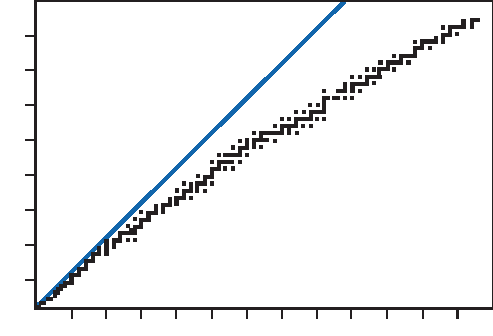
\includegraphics[width=10cm]{../figures/chart-of-nuclides.png}
\captionof{figure}{A schematic `\emph{Chart of Nuclides}' \citep[modified
    from][]{allegre2008}.}
\fi

\section{The age equation}

A characteristic property of radioactive decay is its absolute
independence of external physical and chemical effects. In other
words, it is not affected by changes in pressure, temperature, or the
molecular bonds connecting a radioactive nuclide to neighbouring
atoms. This means that the rate at which a radioactive parent decays
to a radiogenic daughter per unit time, i.e. $dP/dt$ only depends on
$P$, the number of parent atoms present. The \emph{decay constant}
$\lambda$ expresses the likelihood that a radioactive disintegration
takes place in any given time (i.e., $\lambda$ has units of atoms per
atoms per year). This can be expressed mathematically with the
following differential equation:

\begin{equation}
\frac{dP}{dt} = -\lambda P
\label{eq:dPdt}
\end{equation}

Integrating this equation over time yields:

\begin{equation}
P = P_\circ e^{-\lambda t}
\label{eq:P}
\end{equation}

where $P_\circ$ is the number of parent atoms present at time
$t=0$.  Since this number is generally unknown (one exception is
$^{14}$C, see Section \ref{sec:14C}), Equation \ref{eq:P} generally
cannot be used in this form. We can, however, measure the
\emph{present} number of parent and daughter nuclides in the
sample. Rewriting Equation \ref{eq:P}:

\begin{equation}
P_\circ = P e^{\lambda t}
\label{eq:P0}
\end{equation}

and bearing in mind that $P_\circ = P + D$, we obtain:

\begin{equation}
D = P (e^{\lambda t}- 1)
\label{eq:D}
\end{equation}

This equation forms the foundation of most geochronological
methods. It can be rewritten explicitly as a function of time:

\begin{equation}
t = \frac{1}{\lambda} \ln\left(\frac{D}{P} + 1\right)
\label{eq:t}
\end{equation}

The degree of instability of a radioactive nuclide can be expressed by
$\lambda$ or by the \emph{half life} $t_{1/2}$, which is the time
required for half of the parent nuclides to decay. This follows
directly from Equation \ref{eq:P}:

\begin{equation}
\frac{P_\circ}{2} = P_\circ e^{-\lambda t_{1/2}} 
\Rightarrow t_{1/2} = \frac{\ln(2)}{\lambda}
\label{eq:T12}
\end{equation}

As a rule of thumb, the detection limit of a radiometric
geo\-chro\-no\-me\-ter is reached after about 10 half lives. Thus,
$^{14}$C goes back $\sim$50,000 years, $^{10}$Be 10 million and
$^{40}$K 10 billion years.

\section{Decay series}
\label{sec:decay-series}

Sometimes the radiogenic daughter ($D_1$) of a radioactive parent is
radioactive as well, decaying to a daughter of its own ($D_2$), which
may be radioactive again etc., until a stable daughter ($D_*$) is
reached. Considering the simplest case of one intermediate daughter:

\begin{equation}
P \xrightarrow[]{\lambda_P} D_1 \xrightarrow[]{\lambda_1} D_*
\label{eq:series}
\end{equation}

The increase (or decrease) of the number of atoms per unit time for
each of the nuclides is given by:

\begin{align}
\mbox{for~} P &: dP/dt = -\lambda_P P \label{eq:P1}\\
\mbox{for~} D_1 &: dD_1/dt = \lambda_P P - \lambda_1 D_1 \label{eq:D1}\\
\mbox{for~} D_* &: dD_*/dt = \lambda_1 D_1 \label{eq:D*}
\end{align}

The number of parent atoms $P$ can be written as a function of $t$:

\begin{equation}
P = P_\circ e^{-\lambda_P t}
\label{eq:P2}
\end{equation}

Plugging Equation \ref{eq:P2} into \ref{eq:D1} yields

\begin{equation}
dD_1/dt = \lambda_P P_\circ e^{-\lambda_P t} - \lambda_1 D_1
\label{eq:dD1dt}
\end{equation}

Solving this differential equation yields the evolution of $D_1$ with
time. Assuming that $D_1=0$ at $t=0$:

\begin{equation}
D_1 = \frac{\lambda_P}{\lambda_1 - \lambda_P} P_\circ \left[
  e^{-\lambda_P t} - e^{-\lambda_1 t}\right]
\label{eq:ND1}
\end{equation}

If $\lambda_P \ll \lambda_1$ (by a factor of 10 or greater), and $t
\gg 1/\lambda_1$ then $e^{-\lambda_1 t}$ becomes vanishingly small
relative to $e^{-\lambda_P t}$ so that Equation \ref{eq:ND1} can be
simplified:

\begin{equation}
D_1 = \frac{\lambda_P}{\lambda_1 - \lambda_P} P_\circ e^{-\lambda_P t}
\label{eq:ND1b}
\end{equation}

\noindent or, alternatively:

\begin{equation}
D_1 = \frac{\lambda_P}{\lambda_1 - \lambda_P} P
\label{eq:ND1c}
\end{equation}

This means that the ratio of $D_1$ and $P$ remains constant
through time. If $\lambda_P \ll \lambda_1$, then $\lambda_1 -
\lambda_P \approx \lambda_1$, from which it follows that:

\begin{equation}
D_1 = \frac{\lambda_P}{\lambda_1} P
\label{eq:ND1d}
\end{equation}

Rearranging:

\begin{equation}
D_1 \lambda_1 = P \lambda_P
\label{eq:ND1L1}
\end{equation}

or, equivalently:

\begin{equation}
\frac{P}{D_1} = \frac{t_{1/2}(P)}{t_{1/2}(D_1)}
\label{eq:NPND1}
\end{equation}

This is the \emph{secular equilibrium} in which the number of atoms of
both radioactive members is proportional to their respective half
lives. In the geochronological isotope systems $^{235}$U/$^{207}$Pb,
$^{238}$U/$^{206}$Pb and $^{232}$Th/$^{207}$Pb, the lead isotopes are
the end points of a long decay series comprised of several $\alpha$
and $\beta^-$ disintegrations, in which the decay constants of the
parent nuclide is orders of magnitude shorter than the other nuclides
in the chain. For a decay series like that, Equation \ref{eq:ND1L1}
can be generalised to:

\begin{equation}
D_n \lambda_n = \cdots  = D_2 \lambda_2 = D_1 \lambda_1 = P \lambda_P
\label{eq:NDnLn}
\end{equation}

This means that the entire series is in equilibrium, so that all
members occur in mutually constant proportions. The number of atoms of
the stable end member $D_*$ is given by:

\begin{equation}
D_* = P_\circ - P - D_1 - D_2 - \cdots - D_n
\label{eq:ND*}
\end{equation}

Using Equation \ref{eq:NDnLn}, this becomes:

\begin{equation}
D_* = P_\circ - P - \frac{P \lambda_P}{\lambda_1} - 
\frac{P \lambda_P}{\lambda_2} - \cdots - \frac{P \lambda_P}{\lambda_n}
\label{eq:ND*2}
\end{equation}

or

\begin{equation}
D_* = P_\circ - P \left( 1 + \frac{\lambda_P}{\lambda_1} - 
\frac{\lambda_P}{\lambda_2} - \cdots - \frac{\lambda_P}{\lambda_n}\right)
\label{eq:ND*3}
\end{equation}

Since each of the ratios $\lambda_P/\lambda_1$, $\lambda_P/\lambda_2$,
etc.  are vanishingly small, we can simplify Equation \ref{eq:ND*3}
as:

\begin{equation}
D_* = P_\circ - P = P \left( e^{\lambda_P t} -1 \right)
\label{eq:ND*4}
\end{equation}

This means that the accumulation of the final Pb isotope of the
aforementioned three decay series is only a function of the decay of
the parent isotope.  All intermediate decay steps are therefore
inconsequential. In rare cases, however, the isotopic equilibrium is
disturbed by a dissolution or recrystallisation event, say. The
intermediate parent/daughter pairs can then be used to date phenomena
occurring over much shorter time scales than those probed by the U-Pb
method (Section \ref{ch:intro2Useries}).

\begin{figure}[!ht]
  \captionsetup{width=11cm}
  \centering
  \ifpdf
  \ifuclnotes
  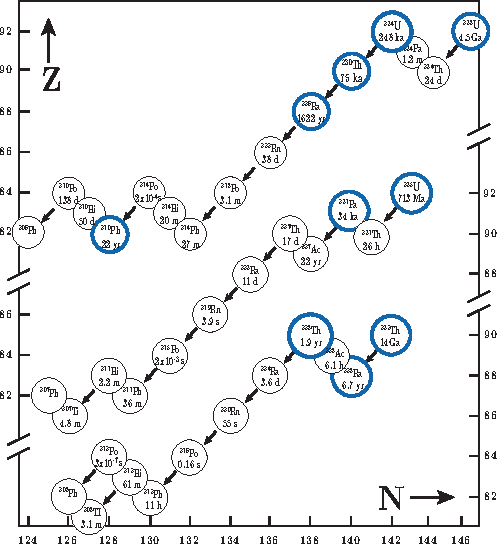
\includegraphics[width=\textwidth]{../figures/U-Th-series.pdf}
  \else
  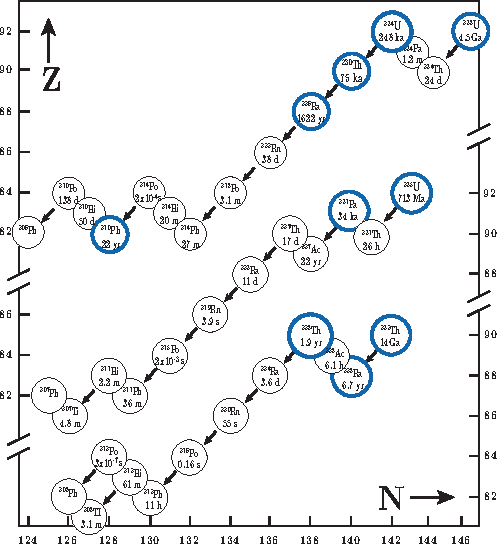
\includegraphics[width=12cm]{../figures/U-Th-series.pdf}
  \fi
  \else
  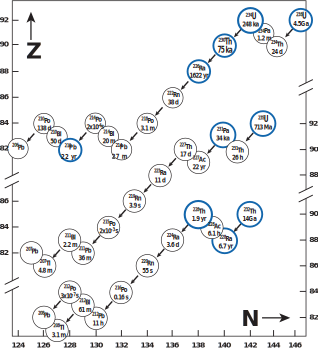
\includegraphics[width=11cm]{../figures/U-Th-series.png}
  \fi
  \caption{The decay series of $^{232}$Th, $^{235}$U and $^{238}$U,
    which form the basis of the U-Th-Pb, U-Th-He and U-Th-series methods
    \citep[modified from][]{allegre2008}.}
  \label{fig:U-Th-series}
\end{figure}


\chapter{Analytical techniques}
\label{ch:analyticaltechniques}

Isotope geochemistry is based on the accurate and precise
determination of elemental and isotopic compositions of rocks and
minerals.  Although some of the earliest geochronological methods
(notably the $^{14}$C method, see Section \ref{sec:14C}) were based on
the detection of radioactivity by means of Geiger-M\"{u}ller counters
and liquid scintillation detectors, nearly all modern isotope
geochemistry is done by mass spectrometry.

\section{Mass spectrometry}
\label{sec:mass-specs}

A mass spectrometer is a device that separates electrically charged
atoms or molecules based on their mass, enabling precise measurement
of the isotopic composition. A mass spectrometer consists of the
following parts:

\begin{enumerate}
\item ion source: this can be either a filament (similar to that found
  in an incandescent light bulb), a plasma torch, a primary ion beam,
  or a spray chamber, among other possibilities.
\item mass analyser: this can be an electromagnet (possibly combined
  with an electrostatic field), or a rapidly fluctuating electric
  field.
\item ion detector: this is, essentially, a volt meter.
\end{enumerate}

In the remainder of this section, we will assume the source to be a
filament and the mass analyser to be an electromagnet. \\

After pumping the mass spectrometer down to (ultra-)high vacuum
conditions (10$^{-6}$ to 10$^{-9}$ mbar), the sample enters the ion
source as a gas, where it is bombarded with electrons.  The resulting
ions (with charge $e$) are accelerated in an electric field (with
potential difference $V$) and collimated to a narrow beam. This beam
is sent through a magnetic field (with strength $H$) which deflects it
into a circular trajectory with a radius proportional to the ion mass
($m$).  This results in a physical separation of the incoming ion beam
into various outgoing beams. The beams of interest are steered into
the ion detector which, in its simplest design (the so-called `Faraday
Cup') consists of a long and narrow cup. The ion beam is neutralised
in the cup by electrons flowing from ground through a resistor. The
potential difference across this resistor is measured and registered
on a computer for further processing.\\

The electric field transfers a certain amount of kinetic energy to the
ions:

\begin{equation}
E = e V = \frac{m v^2}{2}
\label{eq:E}
\end{equation}

With $e$ is the electrical charge (in multiples of 1.60219 $\times
10^{-19}$C, which is the elementary charge of an electron.  Because
each type of ion has a different mass ($m$, in multiples of 1.660538
$\times 10^{-27}$kg, the atomic mass unit), their terminal velocity
($v$) differs as well:

\begin{equation}
v = \sqrt{\frac{2 e V}{m}}
\label{eq:v}
\end{equation}

The mass analyser deflects the ions according to the following equation:

\begin{equation}
H e v = \frac{m v^2}{r}
\label{eq:Hev}
\end{equation}

Substituting Equation \ref{eq:v} into \ref{eq:Hev} yields:

\begin{equation}
H \sqrt{\frac{2 e V}{m}} = \frac{2 V}{r}
\label{eq:H2eVm}
\end{equation}

from which it follows that:

\begin{equation}
\begin{array}{rl}
~ & r = \frac{1}{H}\sqrt{\frac{2 m V}{e}} \\
\mbox{and}~ & H = \frac{1}{r}\sqrt{\frac{2 m V}{e}}\\
\end{array}
\label{eq:rH}
\end{equation}

Equation \ref{eq:rH} allows us to calculate the radius of the ion
trajectory for any given mass-to-charge ratio $m/e$. Note that light
isotopes are more strongly deflected than equally charged heavy ones.
Equation \ref{eq:rH} can also be used to calculate the magnetic field
strength required to deflect an ion beam with a given $m/e$ ratio into
the collector.  This is more practical because most mass spectrometers
have a fixed radius so that the different ions must be collected by
varying $H$. Some modern mass spectrometers are equipped with multiple
ion collectors the enabling simultaneous analysis of several ionic
masses.

\begin{figure}[!ht]
  \centering
  \ifpdf
  \def\svgwidth{\textwidth}
  \input{mass-spec.pdf_tex}
  \else
  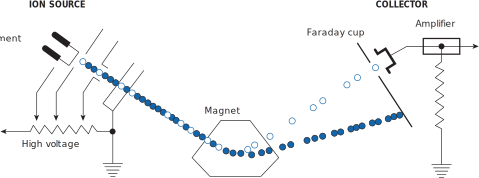
\includegraphics[width=10cm]{../figures/mass-spec.png}
  \fi
  \caption{Schematic diagram of a sector-field noble gas or TIMS mass
    spectrometer \citep[modified from][]{allegre2008}.}
  \label{fig:mass-spec}
\end{figure}

Several types of mass spectrometers are used for geoscience
applications:

\begin{enumerate}
\item{\emph{Thermal Ionisation Mass Spectrometry (TIMS)}.}\\ The
  sample is dissolved and subjected to careful chemical separation
  procedures (liquid chromatography) in order to separate the parent
  and daughter elements to a high level of purity. The resulting
  solutions are spiked and deposited on a tungsten or tantalum
  filament, which is brought to a glow by an electric current and thus
  produces ions. These are separated by a large electromagnet and
  analysed in one or more Faraday cups. TIMS is very time consuming
  but produces extremely precise results (\permil-level precision on
  the ages).
 
\item{\emph{Inductively Coupled Plasma Mass Spectrometry
    (ICP-MS)}.}\\ The sample is vapourised in one of two ways: either
  by introducing a liquid into a spray chamber, or by firing an
  ultraviolet laser at a solid sample and transporting the resulting
  aerosol into the ion source with a carrier gas (typically
  helium). The ion source itself consists of an argon flow which is
  heated to a temperature of approximately 10,000K by sending a
  radiofrequency current through a coil. This breaks up all the
  molecular bonds and produces a plasma (i.e. a `soup' of ions and
  electrons) which enters the high vacuum chamber through a tiny
  opening.  The mass analyser can either be a sector magnet or a
  quadrupole (which consists of four metal rods generating a rapidly
  fluctuating electrical field). ICP-MS offers a higher throughput
  than TIMS, especially in laser ablation mode, where hundreds of ages
  can be measured per day. However, this increased throughput comes at
  the expense of precision, which is on the percent level (better in
  solution mode).

\item{\emph{Secondary ion mass spectrometry (SIMS)}}\\ Prior to the
  development of laser ablation (LA-) ICP-MS, the only other method to
  produce spot measurements in solid samples was by firing a beam of
  negative (e.g. oxygen) or positive (e.g. caesium) ions at the target
  under high vacuum.  This releases (`sputters') positive (or
  negative, in the case of a Cs beam) \emph{secondary} ions from the
  sample surface, which are accelerated by an electrostatic field and
  sent to a sector field mass spectrometer. Although SIMS has been
  replaced by LA-ICP-MS in some applications, it remains an important
  instrument in the geochronological toolbox because (a) it offers
  higher spatial resolution than laser ablation (5-10$\mu m$
  vs. 25-50$\mu m$) and (b) can measure light ions (e.g, hydrogen)
  more reliably than LA-ICP-MS.

\item{\emph{Noble gas mass spectrometry}}\\ The noble gases (He, Ne,
  Ar, Kr, Xe) require a different class of mass spectrometer than the
  rest of the periodic table because, as their name suggests: 1) they
  are gases 2) that do not ionise easily. Noble gasses are liberated
  from solid state materials by heating or laser ablation under
  ultra-high vacuum conditions. To remove any unwanted gas species
  (such as CO, CO\textsubscript{2}, hydrocarbons, etc.) that may
  interfere with the noble gas measurements, the released gas is
  exposed to reactive metals, liquid N\textsubscript{2} `cold traps'
  and other `gettering' devices in a `noble gas extraction line' for a
  duration of 5--30 minutes. The extraction line removes all the
  reactive gas species until only the inert noble gases remain. It is
  only after this lengthy delay that the purified noble gases are
  ionised by electron bombardment, and analysed on the actual mass
  spectrometer.
  
\item{\emph{Accelerator Mass Spectrometer (AMS)}}\\ The AMS combines
  two mass spectrometers with a (`tandem' type) particle accelerator.
  Ions are produced by a SIMS source and steered through a first mass
  analyser, which selects all ions of a desired mass (e.g., mass 14:
  $^{14}$C$^-$, ${}^{12}$CH$_2^-$, $\cdots$). The resulting beam is
  accelerated in the first part of the tandem accelerator by a
  potential difference of several million eV, and sent through a thin
  chamber filled with a `stripper' gas. Collisions of stripper gas
  atoms with the incoming ions destroys any molecular bonds and forms
  3+ ions in the process. The beam now consists of purely atomic ions,
  which are accelerated in the second part of the accelerator and
  steered into a second mass analyser. The AMS has revolutionised the
  $^{14}$C method by enabling the analysis of extremely small
  (mg-sized) samples (see Section \ref{sec:14C}), and has enabled a
  whole new field of geochronology based on the analysis of
  terrestrial cosmogenic radionuclides\ifuclnotes (Chapter
  \ref{sec:cosmo})\fi. The main limitation of AMS is its high
  cost. Currently only two AMS facilities are operating in the UK (in
  Oxford and Glasgow).
\end{enumerate}

\begin{figure}[!ht]
  \centering
  \ifpdf
  \def\svgwidth{\textwidth}
  \input{AMS.pdf_tex}
  \else
  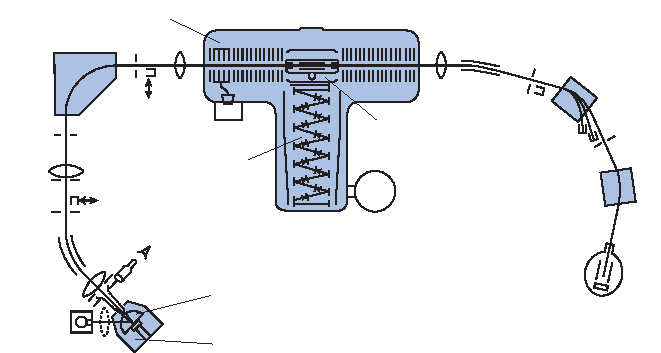
\includegraphics[width=10cm]{../figures/AMS.png}
  \fi
  \caption{Schematic diagram of an Accelerator Mass Spectrometer (AMS)
    \citep[modified from][]{allegre2008}.}
  \label{fig:AMS}
\end{figure}

\section{Isotope dilution}
\label{sec:isotope-dilution}

Besides determining isotopic compositions, the mass spectrometer can
also be used to measure elemental concentrations, using a method
called \emph{isotope dilution}. This is done by mixing the sample
solution (whose isotopic composition has already been determined) with
a known quantity of a solution with a different (but known) isotopic
composition and known elemental concentration. The latter solution is
called the \emph{spike}.  The isotopic composition of the mixture is
analysed by mass spectrometry.  The measured isotopic ratio $R_m$ for
an element with two isotopes ($^aX$ and $^{b}X$) is given by:

\begin{equation}
R_m = \frac{N {}^aX_N + S {}^aX_S}{N {}^bX_N + S {}^bX_S}
\label{eq:Rm}
\end{equation}

with

\begin{equation*}
\begin{array}{rl}
N = & \mbox{the number of atoms of X in the sample}\\
S = & \mbox{the number of atoms of X in the spike}\\
^aX_N, {}^bX_N = & \mbox{the atomic abundance of isotope~} a \mbox{~(or b) in the~}\\
{}^aX_S, {}^bX_S ~~~ & \mbox{sample (or spike)} (^aX_N + {}^bX_N = {}^aX_S + {}^bX_S = 1)
\end{array}
\end{equation*}

$N$ is the only unknown in Equation \ref{eq:Rm}, which can therefore be
rewritten as:

\begin{equation}
N = S \frac{^aX_S - R_m {}^bX_S}{R_m {}^bX_N - {}^aX_N}
\label{eq:N}
\end{equation}

$N$ can also be expressed as a function of the isotopic ratios in the
sample $R_N (={}^aX_N/{}^bX_N)$ and in the spike $R_S
(={}^aX_S/{}^bX_S)$. The atomic abundance of $^aX$ and $^bX$ in the
sample are given by:

\begin{equation}
^aX_N = \frac{R_N}{R_N + 1} \mbox{~and~} {}^bX_N = \frac{1}{R_N + 1}
\label{eq:aXNbXN}
\end{equation}

and in the spike:

\begin{equation}
^aX_S = \frac{R_S}{R_S + 1} \mbox{~and~} {}^bX_S = \frac{1}{R_S + 1}
\label{eq:aXSbXS}
\end{equation}

Substituting Equations \ref{eq:aXSbXS} and \ref{eq:aXNbXN} into
\ref{eq:N} yields:

\begin{equation}
N = S \frac{(R_N+1)(R_S-R_m)}{(R_S+1)(R_m-R_N)}
\label{eq:N2}
\end{equation}

Equations \ref{eq:N} and \ref{eq:N2} give the atomic concentration of
$X$ (in atoms/g).  Dividing $N$ by Avogadro's number $N_A$ and
multiplying with the atomic weights (g/mol) yields the corresponding
weight percentages. Isotope dilution is a very powerful method
because:

\begin{enumerate}
\item It does not require quantative separation of the elements of
  interest.
\item Chemical purification removes unwanted interferences from other
  species.
\item The method is very sensitive, so extremely low concentrations
  can be measured (ppb or less).
\end{enumerate}

\section{Sample-standard bracketing}
\label{sec:bracketing}

Isotope dilution is the `gold standard' for isotope geochemistry,
recommended when the most accurate and precise results are
desired. Unfortunately, isotope dilution is also very time consuming
and cannot be readily applied to micro-analytical techniques such as
LA-ICP-MS and SIMS. In those cases, and alternative method is used,
which is less precise (\%- rather than \permil- level precision) but
quicker.  The idea is to normalise the signal ratios recorded by the
mass spectrometer to a standard of known age.  As before, let P be a
radioactive parent which decays to a radiogenic daughter D. Suppose
that we can measure both nuclides on the same mass spectrometer,
yielding two electronic signal intensities $S_P$ and $S_D$. These
signals may be recorded in units of V, A, or Hz. We cannot directly
use the signal ratios as a proxy for the isotopic ratio:

$$\frac{D}{P} \neq \frac{S_D}{S_P}$$

because the parent and daughter are two different elements with
different chemical properties and ionisation efficiencies. We can,
however, assume that the isotopic ratio is proportional to the signal
ratio:

\begin{equation}
\frac{D}{P} = C \frac{S_D}{S_P}
\label{eq:eqC}
\end{equation}

Thus, if we double $D$ (and thus $D/P$), we would also expect to
double $S_D$ (and thus $S_D/S_P$). To determine the constant of
proportionality $C$, we analyse a standard of known age ($t_s$) and,
hence ($D/P$)-ratio (due to Equation \ref{eq:D}):

\begin{equation}
C = \left(e^{\lambda_Pt_s} - 1\right) \frac{S^s_P}{S^s_D}
\label{eq:const}
\end{equation}

where $\lambda_P$ is the decay constant of the parent and
$S^s_P/S^s_D$ is the (inverse) signal ratio of the standard.


\chapter{Simple parent-daughter pairs}
\label{ch:intro2PD}

\section{$^{14}$C dating}
\label{sec:14C}

There are two stable isotopes of carbon: $^{12}$C and $^{13}$C, and
one naturally occurring radionuclide: $^{14}$C. The half life of
$^{14}$C is only 5,730 years, which is orders of magnitude shorter
than the age of the Earth. Therefore, no primordial radiocarbon
remains and all $^{14}$C is \emph{cosmogenic}\ifuclnotes (see Section
\ref{sec:cosmo} for related methods)\fi.  The main production
mechanism is through secondary cosmic ray neutron reactions with
$^{14}$N in the stratosphere: $^{14}_7$N (n,p) $^{14}_6$C. Any newly
formed $^{14}$C rapidly mixes with the rest of the atmosphere creating
a spatially uniform carbon composition, which is incorporated into
plants and the animals that eat them. Prior to the industrial
revolution, a gram of fresh organic carbon underwent 13.56 ($\beta^-$)
decays per minute. When a plant dies, it ceases to exchange carbon
with the atmosphere and the $^{14}$C concentration decays with time
according to Equation \ref{eq:dPdt}:

\begin{equation}
\frac{d^{14}C}{dt} = -\lambda_{14} \times {}^{14}C
\label{eq:d14Cdt}
\end{equation}

where $\lambda_{14}$ = 0.120968 kyr$^{-1}$. Thus, the radiocarbon
concentration is directly proportional to the radioactivity, which can
be measured by $\beta$-counting. This can then be used to calculate
the radiocarbon age by rearranging Equation \ref{eq:P}:

\begin{equation}
t = -\frac{1}{\lambda_{14}}
\ln\left[\frac{d{}^{14}C/dt}{(d{}^{14}C/dt)_\circ}\right]
\label{eq:t14C}
\end{equation}

where $(d^{14}C/dt)_\circ$ is the original level of $\beta$ activity.
This method was developed by Willard Libby in 1949, for which he was
awarded the Nobel Prize in 1960. As mentioned before,
$(d^{14}C/dt)_\circ$ was 13.56 prior to the industrial revolution,
when thousands of tonnes of `old' carbon were injected into the
atmosphere, resulting in a gradual lowering of the radiocarbon
concentration until 1950, when nuclear testing produced an opposite
effect, leading to a doubling of the atmospheric $^{14}$C activity in
1963. Since the banning of atmospheric nuclear testing, radiocarbon
concentrations have steadily dropped until today, where they have
almost fallen back to their pre-industrial levels. But even prior to
these anthropogenic effects, $^{14}$C concentrations underwent
relatively large fluctuations as a result of secular variations of the
Earth's magnetic field and, to a lesser extent, Solar activity. These
variations in $(d^{14}C/dt)_\circ$ can be corrected by comparison with
a precisely calibrated production rate curve, which was constructed by
measuring the $^{14}$C activity of tree rings
(\emph{dendrochronology}).\\

Since the 1980's, $\beta$-counting has been largely replaced by
accelerator mass spectrometry (AMS, see Section \ref{sec:mass-specs}),
in which the $^{14}$C concentration is measured directly relative to a
stable isotope such as $^{13}$C. Although this has not significantly
pushed back the age range of the radiocarbon method, it has
nevertheless revolutionised the technique by reducing the sample size
requirements by orders of magnitude. It is now possible to analyse
individual seeds or tiny fragments of precious objects such as the
Turin Shroud, which was dated at AD1260-1390.

\section{The Rb-Sr method}
\label{sec:Rb-Sr}

Trace amounts of Rb and Sr are found in most minerals as substitutions
for major elements with similar chemical properties. Rb is an alkali
metal that forms single valent positive ions with an ionic radius of
1.48 \AA, which is similar to K$^+$ (1.33 \AA).  Rb is therefore
frequently found in K-bearing minerals such as micas, K-feldspar and
certain clay minerals. Strongly evolved alkalic rocks such as
syenites, trachites and rhyolites often contain high Rb
concentrations.  Rb contains two isotopes of constant abundance:
$^{85}$Rb (72.1854\%) and $^{87}$Rb (27.8346\%). Sr is an alkaline
earth metal that forms bivalent positive ions with a radius of 1.13
\AA, similar to Ca$^{2+}$ (ionic radius 0.99 \AA). It therefore
substitutes Ca$^{2+}$ in many minerals such as plagioclase, apatite,
gypsum and calcite in sites with 8 neighbours, but not in pyroxene
where Ca$^{2+}$ has a coordination number of 6. Native Sr$^{2+}$ can
also substitute K$^+$ in feldspars (where radiogenic Sr is expected to
be found), but this substitution is limited and requires the
simultaneous replacement of Si$^{4+}$ by Al$^{3+}$ in order to
preserve electric neutrality.  Sr therefore predominantly occurs in
Ca-rich undifferentiated rocks such as basalts. Sr contains four
isotopes ($^{84}$Sr, $^{86}$Sr, $^{87}$Sr and $^{88}$Sr) with variable
abundance due to the variable amount of radiogenic $^{87}$Sr. However,
the non-radiogenic $^{84}$Sr/$^{86}$Sr and $^{86}$Sr/$^{88}$Sr-ratios
are constant with values of 0.056584 and 0.1194, respectively. The
Rb-Sr chronometer is based on the radioactive decay of $^{87}$Rb to
$^{87}$Sr:

\begin{equation}
{}^{87}Rb \rightarrow {}^{87}Sr + \beta^- + \nu +
0.275 MeV
\label{eq:87Rb}
\end{equation}

Where $\nu$ indicates an antineutrino. The number of radiogenic
${}^{87}$Sr atoms produced by this reaction after a time t is given
by:

\begin{equation}
{}^{87}Sr^* = {}^{87}Rb (e^{\lambda_{87} t} - 1)
\label{eq:87Sr*}
\end{equation}

where $^{87}Rb$ is the actual number of $^{87}$Rb atoms per unit
weight and $\lambda_{87}$ is the decay constant 1.42 $\times$
10$^{-11}$ yr$^{-1}$ (t$_{1/2}$ = 4.88$\times$10$^{10}$yr).  In
addition to this radiogenic $^{87}$Sr, most samples will also contain
some `ordinary' Sr. The total number of $^{87}$Sr atoms measured is
therefore given by:

\begin{equation}
^{87}Sr = {}^{87}Sr^* + {}^{87}Sr_\circ
\label{eq:87Sr}
\end{equation}

with $^{87}Sr_\circ$ the initial $^{87}$Sr present at the time of
isotopic closure.  Combining Equations \ref{eq:87Sr} and
\ref{eq:87Rb}, we obtain:

\begin{equation}
^{87}Sr = {}^{87}Sr_\circ + {}^{87}Rb (e^{\lambda_{87} t} - 1)
\label{eq:87Sr2}
\end{equation}

Dividing this by the non-radiogenic $^{86}$Sr yields

\begin{equation}
\frac{^{87}Sr}{^{86}Sr} =
\left(\frac{^{87}Sr}{^{86}Sr}\right)_\circ +
\frac{^{87}Rb}{^{86}Sr} (e^{\lambda_{87} t} - 1)
\label{eq:87Sr86Sr}
\end{equation}

The method can be applied to single minerals or to whole rocks.  Given
the very long half life, the optimal time scale ranges from the
formation of the solar system to the late Palaeozoic (300-400 Ma).  To
measure a Rb/Sr age, the weight percentage of Rb is measured by means
of X-ray fluorescence, ICP-OES or similar techniques, and the
$^{87}$Sr/$^{86}$Sr ratio is determined by mass spectrometry (isotope
dilution). The $^{87}$Rb/$^{86}$Sr-ratio is then calculated as:

\begin{equation}
\frac{^{87}Rb}{^{86}Sr} =
\frac{Rb}{Sr} \frac{Ab(^{87}Rb)
  M(Sr)}{Ab(^{86}Sr) M(Rb)}
\label{eq:87Rb86Sr}
\end{equation}

Where $Ab(\cdot)$ signifies `abundance' and $M(\cdot)$ `molar mass'.

\section{Isochrons}
\label{sec:isochrons}

Equation \ref{eq:87Rb86Sr} can be used in one of two ways. A first
method is to use an assumed value for $(^{87}$Sr$/^{86}$Sr)$_\circ$,
based on the geological context of the sample. This method is only
reliable for samples with a high Rb/Sr ratio (e.g., biotite) because
in that case, a wrong value for $({}^{87}$Sr$/{}^{86}$Sr$)_\circ$ has
only a minor effect on the age. A second and much better method is to
analyse several minerals of the same sample and plot them on a
$(^{87}$Rb$/^{86}$Sr) vs.  (${}^{87}$Sr$/{}^{86}$Sr) diagram (Figure
\ref{fig:isochron}).  Due to Equation \ref{eq:87Sr86Sr}, this should
form a linear array (the so-called \emph{isochron}) with slope
$(e^{\lambda_{87} t} - 1)$ and intercept
$({}^{87}Sr/{}^{86}Sr)_\circ$.  Both parameters can be determined
by linear regression, allowing us to quantify the `goodness of fit' of
the data and obviating the need to assume any initial Sr-ratios.

\ifpdf
\ifuclnotes
\begin{figure}[!ht]
  \centering
  \def\svgwidth{.7\textwidth}
  \input{isochron.pdf_tex}
  \caption{Schematic evolution of the $^{87}$Sr$/{}^{86}$Sr-system as
    a function of time for multiple aliquots of a hypothetical sample
    with initial ratio $({}^{87}$Sr$/{}^{86}$Sr$)_\circ$=0.700. The
    slope of the isochron is a function of the age as per Equation
    \ref{eq:87Sr86Sr} \citep[modified from][]{allegre2008}.}
  \label{fig:isochron}
\end{figure}
\else % end of uclnotes
\begin{figure}[!ht]
\noindent\begin{minipage}[t]{.6\textwidth}
\strut\vspace*{-\baselineskip}\newline
\def\svgwidth{\textwidth}
\input{isochron.pdf_tex}
\end{minipage}
\begin{minipage}[t]{.4\textwidth}
  \captionof{figure}{Schematic evolution of the $^{87}$Sr$/{}^{86}$Sr-system as
    a function of time for multiple aliquots of a hypothetical sample
    with initial ratio $({}^{87}$Sr$/{}^{86}$Sr$)_\circ$=0.700. The
    slope of the isochron is a function of the age as per Equation
    \ref{eq:87Sr86Sr} \citep[modified from][]{allegre2008}.}
  \label{fig:isochron}
\end{minipage}
\end{figure}
\fi % end of pdf
\else
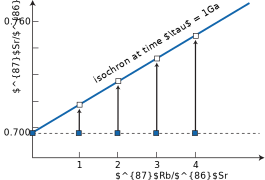
\includegraphics[width=10cm]{../figures/isochron.png}
  \captionof{figure}{Schematic evolution of the $^{87}$Sr$/{}^{86}$Sr-system as
    a function of time for multiple aliquots of a hypothetical sample
    with initial ratio $({}^{87}$Sr$/{}^{86}$Sr$)_\circ$=0.700. The
    slope of the isochron is a function of the age as per Equation
    \ref{eq:87Sr86Sr} \citep[modified from][]{allegre2008}.}
  \label{fig:isochron}
\fi

\section{The Sm-Nd method}
\label{sec:Sm-Nd}

The elements Neodymium (Z=60) and Samarium (Z=62) are so-called `rare
earth elements'.  All elements of this family have similar chemical
properties. They nearly all form 3+ ions of roughly equal albeit
slightly decreasing size with atomic number.  The ionic radius of Nd
and Sm is 1.08 and 1.04 \AA, respectively.  As the name suggests, rare
earth elements rarely form the major constituents of minerals.  One
notable exception is monazite, which is a rare earth phosphate. In
most cases, the rare earth elements are found in trace amounts of up
to 0.1\% in apatite [Ca$_5$(PO$_4$)$_3$(OH,Cl,F)] and zircon
[ZrSiO$_4$]. Both Sm and Nd are slightly enriched in feldspar, biotite
and apatite and thus tend to be found in higher concentrations in
differentiated (alkalic) magmatic rocks.\\

Because their chemical properties are so similar, geological processes
are rarely capable of fractionating the Sm and Nd
concentrations. Therefore, the Sm/Nd ratio in most rocks generally
falls in a narrow range of 0.1 to 0.5 (the Sm/Nd ratio of the solar
system being 0.31). One exception is garnet, in which Sm/Nd ratios $>$
1 have been found. Partial melting of mafic minerals such as pyroxene
and olivine produces lower Sm/Nd ratios in the fluid phase than the
solid residue.  The Sm/Nd ratio of magmatic rocks therefore decreases
with increasing differentiation.\\

Natural Sm contains seven naturally occurring isotopes, three of which
are radioactive ($^{147}$Sm, $^{148}$Sm and $^{149}$Sm). Only
$^{147}$Sm has a sufficiently short half life to be useful for
geochronology.  Nd also contains seven isotopes, of which only one is
radioactive ($^{144}$Nd) but with a very long half life. $^{143}$Nd is
the radiogenic daughter of $^{147}$Sm and is formed by
$\alpha$-decay. This forms the basis of the Sm-Nd chronometer.
Analogous to the Rb-Sr method (Equation \ref{eq:87Sr*}), we can write:

\begin{equation}
^{143}Nd^* = {}^{147}Sm (e^{\lambda_{147} t} - 1)
\label{eq:144Nd*}
\end{equation}

Hence:

\begin{equation}
t = \frac{1}{\lambda_{147}}
\ln\left(\frac{^{143}Nd^*}{^{147}Sm} + 1 \right)
\label{eq:tNd}
\end{equation}

With $\lambda_{147}$ = 6.54$\times$10$^{-12} $yr$^{-1}$ ($t_{1/2}$ =
1.06$\times$10$^{11}$yr).  Since most samples contain some initial Nd,
the preferred way to calculate Sm/Nd ages is by analysing several
minerals in a rock and create an isochron, similar to the Rb/Sr method
(Section \ref{sec:isochrons}):

\begin{equation}
\frac{^{143}Nd}{^{144}Nd} =
\left(\frac{^{143}Nd}{^{144}Nd}\right)_{\circ} +
\frac{^{147}Sm}{^{144}Nd} \left(e^{\lambda_{147}t} -
1\right)
\label{eq:143Nd147Nd}
\end{equation}

All measurements are done by mass spectrometry using isotope dilution.
Because of the identical atomic masses of $^{147}$Sm and $^{147}$Nd,
it is necessary to perform a chemical separation between Sm and Nd
prior to analysis.\\

The Sm/Nd method is generally applied to basic and ultrabasic igneous
rocks (basalt, peridotite, komatiite) of Precambrian to Palaeozoic
age. The method thus complements the Rb/Sr method, which is
preferentially applied to acidic rock types. The Sm/Nd method can also
be applied to high grade metamorphic rocks (granulites, eclogites) as
well as meteorites (shergottites, nahklites). Since the rare earths
are significantly less mobile than Rb and Sr, the Sm/Nd is more
reliable in rocks that have been disturbed by weathering or
metamorphism.


\chapter{The U-Pb system}
\label{sec:U-Pb}

U and Th are found on the extremely heavy end of the Periodic Table of
Elements.  All their isotopes are radioactive and exhibit
$\alpha$-decay and sometimes even spontaneous fission (see Section
\ref{sec:fission-tracks}). $^{232}$Th, $^{235}$U and $^{238}$U each
form the start of long decay series comprising multiple $\alpha$- and
$\beta$ emissions which eventually produce various isotopes of Pb:

\begin{equation}
\begin{array}{rl}
^{238}U \rightarrow & {}^{206}Pb + 8\alpha + 6\beta + 47\mbox{MeV} \\ 
^{235}U \rightarrow & {}^{207}Pb + 7\alpha + 4\beta + 45\mbox{MeV} \\
^{232}Th \rightarrow & {}^{208}Pb + 6\alpha + 4\beta + 40\mbox{MeV} 
\end{array}
\label{eq:UThdecay}
\end{equation}

Each of these three decay series is unique, i.e. no isotope occurs in
more than one series (Figure \ref{fig:U-Th-series}). Furthermore, the
half life of the parent isotope is much longer than any of the
intermediary daughter isotopes, thus fulfilling the requirements for
secular equilibrium (Section \ref{sec:decay-series}). We can therefore
assume that the $^{206}$Pb is directly formed by the $^{238}$U, the
$^{207}$Pb from the $^{235}$U and the $^{208}$Pb from the
$^{232}$Th. Several chronometers are based on the $\alpha$-decay of U
and Th:

\begin{itemize}
\item The U-Th-Pb method (Section \ref{sec:U-Th-Pb})
\item The Pb-Pb method (Section \ref{sec:Pb-Pb})
\item The U-Th-He method (Section \ref{sec:U-Th-He})
\end{itemize}

\section{The U-(Th-)Pb method}
\label{sec:U-Th-Pb}

Natural Pb consists of four isotopes $^{204}$Pb, $^{206}$Pb,
$^{207}$Pb and $^{208}$Pb. The ingrowth equations for
the three radiogenic Pb isotopes are given by:

\begin{equation}
  \begin{array}{rl}
    &{}^{206}Pb^* = {}^{238}U \left(e^{\lambda_{238}t} - 1\right)\\ 
    &{}^{207}Pb^* = {}^{235}U \left(e^{\lambda_{235}t} - 1\right)\\ 
    &{}^{208}Pb^* = {}^{232}Th \left(e^{\lambda_{232}t} - 1\right)
  \end{array}
  \label{eq:Pb*}
\end{equation}

With $\lambda_{238}$ = 1.55125 $\times 10^{-10} a^{-1}$ (t$_{1/2}$ =
4.468 Gyr), $\lambda_{235}$ = 9.8485 $\times 10^{-10} a^{-1}$
(t$_{1/2}$ = 703.8 Myr), and $\lambda_{232}$ = 0.495 $\times 10^{-10}
a^{-1}$ (t$_{1/2}$ = 14.05 Gyr). The corresponding age equations are:

\begin{equation}
  \begin{array}{rl}
    t_{206} & = \frac{1}{\lambda_{238}}
    \ln \left(\frac{{}^{206}Pb^*}{{}^{238}U}+1\right)\\
    t_{207} & = \frac{1}{\lambda_{235}}
    \ln \left(\frac{{}^{207}Pb^*}{{}^{235}U}+1\right)\\
    t_{208} & = \frac{1}{\lambda_{232}}
    \ln \left(\frac{{}^{208}Pb^*}{{}^{232}Th}+1\right)
  \end{array}
  \label{eq:tPb*}
\end{equation}

Some igneous minerals (notably zircon) conveniently incorporate lots
of U and virtually no Pb upon crystallisation. For those minerals, the
non-radiogenic Pb can be safely neglected (at least for relatively
young ages), so that we can assume that $Pb \approx Pb^*$. This
assumption cannot be made for other minerals, young ages, and high
precision geochronology. In those cases, the inherited component (aka
`common Pb') needs to be quantified, which is done by normalising to
non-radiogenic $^{204}$Pb:

\begin{equation}
\begin{array}{c}
  \frac{^{206}Pb}{^{204}Pb} = \left(\frac{^{206}Pb}{^{204}Pb}\right)_\circ +
  \frac{^{238}U}{^{204}Pb} \left(e^{\lambda_{238}t} - 1\right) \\
  \frac{^{207}Pb}{^{204}Pb} = \left(\frac{^{207}Pb}{^{204}Pb}\right)_\circ +
  \frac{^{235}U}{^{204}Pb} \left(e^{\lambda_{235}t} - 1\right)\\
  \frac{^{208}Pb}{^{204}Pb} = \left(\frac{^{208}Pb}{^{204}Pb}\right)_\circ +
  \frac{^{232}Th}{^{204}Pb} \left(e^{\lambda_{232}t} - 1\right)
\end{array}
\label{eq:Pb}
\end{equation}

where $\left(\frac{^{x}Pb}{^{204}Pb}\right)_\circ$ stands for the
common Pb component for isotope x. The corresponding age equations
then become:

\begin{equation}
\begin{array}{c}
  t_{206}=\frac{1}{\lambda_{238}}\ln\left(\frac{\left(\frac{^{206}Pb}{^{204}Pb}\right)-
    \left(\frac{^{206}Pb}{^{204}Pb}\right)_\circ}{\frac{^{238}U}{^{204}Pb}}+1\right)\\
  t_{207}=\frac{1}{\lambda_{235}}\ln\left(\frac{\left(\frac{^{207}Pb}{^{204}Pb}\right)-
    \left(\frac{^{207}Pb}{^{204}Pb}\right)_\circ}{\frac{^{235}U}{^{204}Pb}}+1\right)\\
  t_{208}=\frac{1}{\lambda_{232}}\ln\left(\frac{\left(\frac{^{208}Pb}{^{204}Pb}\right)-
    \left(\frac{^{208}Pb}{^{204}Pb}\right)_\circ}{\frac{^{232}Th}{^{204}Pb}}+1\right)
\end{array}
\label{eq:tPb}
\end{equation}

U-Pb dating grants access to two separate geochronometers
($^{206}$Pb/${}^{238}$U and $^{207}$Pb/${}^{235}$U) based on different
isotopes of the same parent-daughter pair (i.e. U \& Pb).  This
built-in redundancy provides a powerful internal quality check which
makes the method arguably the most robust and reliable dating
technique in the geological toolbox. The initial Pb composition can
either be determined by analysing the Pb composition of a U-poor
mineral (e.g., galena or feldspar) or by applying the isochron method
to samples with different U and Th concentrations. As is the case for
any isotopic system, the system needs to remain `closed' in order to
yield meaningful isotopic ages.  This sometimes is not the case,
resulting in a loss of Pb and/or U.  Such losses cause the
$^{206}$Pb/$^{238}$U- and $^{207}$Pb/$^{235}$U-clocks to yield
different ages. Note that isotopic closure is required for all
intermediary isotopes as well.  Critical isotopes are the highly
volatile $^{226}$Rn (t$_{1/2}$=1.6ka) and $^{222}$Rn
(t$_{1/2}$=3.8d). Initially, the U-Pb method was applied to U-ores,
but nowadays it is predominantly applied to accessory minerals such
zircon and, to a lesser extent, apatite, monazite and allanite.

\section{The Pb-Pb method}
\label{sec:Pb-Pb}

The $^{207}$Pb/$^{206}$Pb method is based on the U-Pb method and is
obtained by dividing the two U-Pb members of Equation \ref{eq:Pb*} (or
\ref{eq:Pb}), and taking into account that the average natural
$^{238}$U/$^{235}$U-ratio is 137.818:

\begin{equation}
\frac{^{207}Pb^*}{^{206}Pb^*} = 
\frac{\left(\frac{^{207}Pb}{^{204}Pb}\right)-\left(\frac{^{207}Pb}{^{204}Pb}\right)_\circ}
{\left(\frac{^{206}Pb}{^{204}Pb}\right)-\left(\frac{^{206}Pb}{^{204}Pb}\right)_\circ}
= \frac{1}{137.818} \frac{e^{\lambda_{235}t}-1}{e^{\lambda_{238}t}-1}
\label{eq:PbPb}
\end{equation}

The left hand side of this equation contains only Pb isotopic ratios.
Note that these are \emph{only} a function of time. Equations
\ref{eq:PbPb} has no direct solution and must be solved
iteratively. The Pb-Pb method has the following advantages over
conventional U-Pb dating:

\begin{itemize}
\item There is no need to measure uranium.
\item The method is insensitive to recent loss of U and even Pb,
  because this would not affect the isotopic ratio of the Pb.
\end{itemize}

In practice, the Pb-Pb method is rarely applied by itself but is
generally combined with the U-Pb technique. The expected
$({}^{207}Pb/{}^{206}Pb)^*$-ratio for recently formed rocks and minerals
can be calculated from Equation \ref{eq:PbPb} by setting
t$\rightarrow$0:

\begin{equation}
  \left(\frac{^{207}Pb}{^{206}Pb}\right)^*_p =
  \frac{\lambda_{235}}{137.818\lambda_{238}} = 0.04607
\label{eq:commonPb}
\end{equation}

This ratio was progressively higher as one goes back further in time.
It was $\approx$ 0.6 during the formation of Earth.

\section{Concordia}
\label{sec:intro2concordia}

It sometimes happens that the U-Th-Pb trio of chronometers does not
yield mutually consistent ages. It is then generally found that
t$_{208}$ $<$ t$_{206}$ $<$ t$_{207}$ $<$ t$_{207/206}$ which, again,
shows that the Pb-Pb clock is least sensitive to open system
behaviour.  From Equation \ref{eq:Pb*}, we find that:

\begin{equation}
\begin{array}{rl}
\frac{^{206}Pb^*}{^{238}U} & = e^{\lambda_{238}t}-1 \mbox{~and}\\
\frac{^{207}Pb^*}{^{235}U} & = e^{\lambda_{235}t}-1
\end{array}
\label{eq:wetherill}
\end{equation}

If we plot those $^{206}$Pb$^*$/$^{238}$U- and
$^{207}$Pb$^*$/$^{235}$U-ratios which yield the same ages (t) against
one another, they form a so-called `concordia' curve. The concordia
diagram is a very useful tool for investigating and interpreting
disruptions of the U-Pb system caused by `episodic lead loss'. This
means that a mineral (of age T$_\circ$, say) has lost a certain
percentage of its radiogenic Pb at a time T$_1$ after its formation
(e.g., during metamorphism), after which the system closes again and
further accumulation of radiogenic Pb proceeds normally until the
present.  On the concordia diagram of multiple aliquots of a sample,
this scenario will manifest itself as a linear array of datapoints
connecting the concordant $^{206}$Pb$^*$/$^{238}$U -
$^{207}$Pb$^*$/$^{235}$U composition expected at T$_\circ$ with that
expected at T$_1$.  With time, the data shift further away from the
origin.  The upper intercept of the linear array (aka \emph{discordia}
line) can be used to estimate the crystallisation age, whereas the
lower intercept yields the age of metamorphism.  The greater the
distance from the expected composition at t, the greater the degree of
Pb loss and the greater the linear extrapolation error on the
crystallisation age (Figure \ref{fig:wetherill}).

\ifpdf
\ifuclnotes
\begin{figure}[!ht]
  \centering
  \def\svgwidth{.7\textwidth}
  \input{wetherill.pdf_tex}
  \caption{`Wetherill' concordia diagram showing concordant (filled
    symbols) and discordant (empty symbols) analyses affected by
    different degrees of Pb (or U) loss \citep[modified
      from][]{allegre2008}.}
  \label{fig:wetherill}
\end{figure}
\else % end of uclnotes
\begin{figure}[!ht]
\noindent\begin{minipage}[t]{.5\textwidth}
\strut\vspace*{-\baselineskip}\newline
\def\svgwidth{\textwidth}
\input{wetherill.pdf_tex}
\end{minipage}
\begin{minipage}[t]{.5\textwidth}
\captionof{figure}{`Wetherill' concordia diagram showing concordant
  (filled symbols) and discordant (empty symbols) analyses affected by
  different degrees of Pb (or U) loss \citep[modified
    from][]{allegre2008}.}
  \label{fig:wetherill}
\end{minipage}
\end{figure}
\fi % end of pdf
\else

\includegraphics[width=10cm]{../figures/wetherill.png}
\captionof{figure}{`Wetherill' concordia diagram showing concordant
  (filled symbols) and discordant (empty symbols) analyses affected by
  different degrees of Pb (or U) loss \citep[modified
    from][]{allegre2008}.}
  \label{fig:wetherill}
\fi

\section{Detrital geochronology}

Zircon (ZrSiO$_4$) is a common U-Th-bearing accessory mineral in
acidic igneous rocks, which form the main proto-sources of the
siliciclastic sediments. Zircon is a very durable mineral that
undergoes minimal chemical alteration or mechanical
abrasion. Therefore, zircon crystals can be considered time capsules
carrying the igneous and metamorphic history of their
proto-sources. The probability distribution of a representative sample
of zircon U-Pb ages from a detrital population can serve as a
characteristic fingerprint that may be used to trace the flow of sand
through sediment routing systems. As a provenance tracer, zircon U-Pb
data are less susceptible to winnowing effects than conventional
petrographic techniques. Using modern microprobe technology (SIMS and
LA-ICP-MS, see Chapter \ref{sec:mass-specs}), it is quite easy to
date, say, a hundred grains of zircon in a matter of just a few
hours. Due to the robustness of zircons as a tracer of sedimentary
provenance, and the relative ease of dating them, the use of detrital
zircon U-Pb geochronology has truly exploded in recent years. A
literature survey using the keywords `detrital', `zircon', and
`provenance' indicates that the proliferation of detrital zircon
studies has followed an exponential trend, with the number of
publications doubling roughly every five years over the past two
decades. At present, nearly a thousand detrital zircon publications
appear each year.\\

An extensive survey of late Archaean sandstones from the Jack Hills in
Australia have revealed a subpopulation of detrital zircons with
Hadean (4.1-4.2 Ga) U-Pb ages. These are the oldest terrestrial
minerals known to science, predating the oldest igneous rocks by 300
million years.  The isotopic composition of oxygen, hafnium and other
elements in the zircon represents a unique window into the earliest
stages of Earth evolution.  They indicate that liquid water was
present on the surface of our planet early on in its history. This
isotopic evidence is corroborated by the geological observation that
the Hadean zircons are preserved in fluvial deposits.


\chapter{The K-Ar system}
\label{sec:K-Ar}

Potassium has three naturally occurring isotopes: $^{39}$K, $^{40}$K
and $^{41}$K. $^{40}$K is radioactive and undergoes branched decay to
$^{40}$Ca (by electron emission $\lambda_{\beta-} = 4.962 \times
10^{-10} yr^{-1}$) and $^{40}$Ar (by electron capture $\lambda_{e} =
0.581 \times 10^{-10} yr^{-1}$) with a combined half life of 1.248
billion years. The positron emission mechanism mentioned in Chapter
\ref{sec:radioactivity} has an extremely long half life and can
therefore safely be neglected. In addition to $^{40}$Ar, argon has two
more stable isotopes: $^{36}$Ar and $^{38}$Ar. Argon makes up
$\sim$1\% of the terrestrial atmosphere, with a fixed isotopic
composition of $^{40}$Ar/$^{36}$Ar = 298.5 and $^{38}$Ar/$^{36}$Ar =
0.187. The argon contained in K-bearing minerals is made up of a
mixture of radiogenic ($^{40}$Ar$^*$) and non-radiogenic gas
($^{40}$Ar$_\circ$):

\begin{equation}
\begin{array}{rl}
^{40}Ar & = {}^{40}Ar_\circ + {}^{40}Ar^*\\ 
\mbox{where~} {}^{40}Ar^* & =
  \frac{\lambda_e}{\lambda} {}^{40}K \left( e^{\lambda t} - 1 \right)
\end{array}
\label{eq:Ar}
\end{equation}

with $\lambda$ the total decay constant of $^{40}$K ($\lambda =
\lambda_e + \lambda_{\beta-}$ = $5.543 \times 10^{-10} yr^{-1}$).

\section{K-Ar dating}

The $^{40}$K $\rightarrow$ $^{40}$Ar$^*$ decay scheme forms the basis
of the K-Ar geochronometer, with the following age equation:

\begin{equation}
t = \frac{1}{\lambda} \ln\left[ 1 + \frac{\lambda}{\lambda_e}
  \left(\frac{^{40}Ar^*}{^{40}K}\right) \right]
\label{eq:K-Ar}
\end{equation}

Taking into account the `contaminated' (aka `excess' or `inherited')
argon component $^{40}Ar_\circ$ and analysing several cogenetic rocks
or minerals with different K (and therefore $^{40}Ar^*$) contents, an
\emph{isochron} equation can be formed by division through $^{36}$Ar:

\begin{equation}
\frac{^{40}Ar}{^{36}Ar} = \left(\frac{^{40}Ar}{^{36}Ar}\right)_\circ +
\frac{\lambda_e}{\lambda} \frac{^{40}K}{^{36}Ar} \left( e^{\lambda t} - 1 \right)
\label{eq:K-Ar-isochron}
\end{equation}

which can be solved for t. Alternatively, we can simply assume that
all the inherited argon has an atmospheric origin, so that
$({}^{40}Ar/{}^{36}Ar)_\circ = 298.5$.

\section{$^{40}$Ar/$^{39}$Ar dating}
\label{sec:Ar-Ar}

From an analytical perspective, K-Ar dating is a two step
process. Because K (an alkali metal) and Ar (a noble gas) cannot be
measured on the same analytical equipment, they must be analysed
separately on two different aliquots of the same sample.  This
limitation is overcome by the $^{40}$Ar/$^{39}$Ar technique, which is
a clever variation of the K-Ar method. The idea is to subject the
sample to neutron irradiation and convert a small fraction of the
$^{39}$K to synthetic $^{39}$Ar, which has a half life of 269
years. The age equation can then be rewritten as follows:

\begin{equation}
t_x = \frac{1}{\lambda} \ln\left[
1 + J \left(\frac{^{40}Ar^*}{^{39}Ar}\right)_x 
\right]
\label{eq:Ar-Ar}
\end{equation}

where `x' stands for `sample' and J is a constant of proportionality
which encapsulates the efficiency of the $^{39}$K (n,p) $^{39}$Ar
reaction and into which the factor $\lambda/\lambda_e$ is folded as
well.  The J-value can be determined by analysing a standard of known
age t$_s$ which was co-irradiated with the sample:

\begin{equation}
t_s = \frac{1}{\lambda} \ln\left[
1 + J \left(\frac{^{40}Ar^*}{^{39}Ar}\right)_s 
\right]
\label{eq:J}
\end{equation}

In which the subscript `s' stands for `standard'. The great advantage
of equation \ref{eq:Ar-Ar} over \ref{eq:K-Ar} is that all measurements
can be completed on the same aliquot and using a single instrument,
namely a noble gas mass spectrometer, which can analyse extremely
small (down to $\mu$g-sized) samples.\\

The $^{40}$Ar/$^{39}$Ar-method also allows the analyst to investigate
the extent of \emph{argon loss} by means of stepwise heating
experiments.  This is done by degassing the sample under ultra-high
vacuum conditions in a resistance furnace. At low temperatures, the
weakly bound Ar is released, whereas the strongly bound Ar is released
from the crystal lattice at high temperatures until the sample
eventually melts. Plotting the \emph{apparent ages} against the
cumulative fraction of $^{39}$Ar released yields an
$^{40}$Ar/$^{39}$Ar age spectrum (Figure \ref{fig:Ar-Ar}).  If a rock
or mineral has remained closed since its formation, the
$^{40}$Ar/$^{39}$Ar-ratio should remain constant over the course of
the different heating steps, forming an `age plateau'. More complex
(e.g. rising) release spectra, on the other hand, are diagnostic of
complex thermal histories featuring partial argon loss. `saddle'
shaped release spectra are indicative of `excess' argon. The
composition of the inherited argon gas can be determined using a
variant of the isochron method, assuming that all ${}^{36}Ar$ is
inherited:

\begin{equation}
\frac{{}^{40}Ar}{{}^{36}Ar} =
\left(\frac{{}^{40}Ar}{{}^{36}Ar}\right)_\circ +
\frac{{}^{39}Ar}{{}^{36}Ar}\frac{e^{\lambda t} - 1}{J}
\label{eq:Ar-Ar-isochron}
\end{equation}

If the Ar contamination is constant throughout the entire sample, then
the $\frac{^{40}Ar}{^{36}Ar}$-measurements will be arranged along a
linear trend whose slope is a function of $\frac{^{40}Ar^*}{^{39}Ar}$
and, hence, the age.\\

\ifpdf
\ifuclnotes
\begin{figure}[!ht]
  \centering
  \def\svgwidth{.7\textwidth}
  \input{Ar-Ar.pdf_tex}
  \caption{$^{40}$Ar/$^{39}$Ar age spectra obtained by stepwise
    heating of three different K-bearing minerals. Biotite exhibits a
    flat `plateau', indicating a simple history of rapid
    crystallisation and/or cooling. K-feldspar shows a rising age
    spectrum, consistent with a more complex evolution comprising
    multiple growth phases and/or thermal resetting. Finally,
    hornblende shows a `U-shaped' release spectrum in which the first
    heating step releases a large amount of `excess' argon
    \citep[modified from][]{allegre2008}.}
  \label{fig:Ar-Ar}
\end{figure}
\else % end of uclnotes
\begin{figure}[!ht]
\noindent\begin{minipage}[t]{.55\textwidth}
\strut\vspace*{-\baselineskip}\newline
\def\svgwidth{\textwidth}
\input{Ar-Ar.pdf_tex}
\end{minipage}
\begin{minipage}[t]{.45\textwidth}
  \captionof{figure}{$^{40}$Ar/$^{39}$Ar age spectra obtained by stepwise
    heating of three different K-bearing minerals. Biotite exhibits a
    flat `plateau', indicating a simple history of rapid
    crystallisation and/or cooling. K-feldspar shows a rising age
    spectrum, consistent with a more complex evolution comprising
    multiple growth phases and/or thermal resetting. Finally,
    hornblende shows a `U-shaped' release spectrum in which the first
    heating step releases a large amount of `excess' argon
    \citep[modified from][]{allegre2008}.}
  \label{fig:Ar-Ar}
\end{minipage}
\end{figure}
\fi % end of pdf
\else
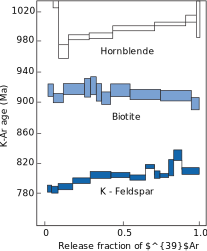
\includegraphics[width=10cm]{../figures/Ar-Ar.png}
  \captionof{figure}{$^{40}$Ar/$^{39}$Ar age spectra obtained by stepwise
    heating of three different K-bearing minerals. Biotite exhibits a
    flat `plateau', indicating a simple history of rapid
    crystallisation and/or cooling. K-feldspar shows a rising age
    spectrum, consistent with a more complex evolution comprising
    multiple growth phases and/or thermal resetting. Finally,
    hornblende shows a `U-shaped' release spectrum in which the first
    heating step releases a large amount of `excess' argon
    \citep[modified from][]{allegre2008}.}
  \label{fig:Ar-Ar}
\fi

\section{Applications}
\label{sec:Ar-applications}

The K-Ar and $^{40}$Ar/$^{39}$Ar-methods are some of the most widely
used geochronometers and important tools in the calibration of the
geologic time scale. The method is applicable to rocks and minerals
$>$ 10$^6$yr. Obviously, younger materials require more careful
treatment of the inherited argon components.

\begin{itemize}
\item{Magmatic rocks:} formation ages can only be obtained for rapidly
  cooled volcanic rocks, using either mineral separates (sanidine,
  biotite, hornblende) or whole rocks. Pyroclastics and obsidian may
  yield reliable ages only if they are unaltered and contain little
  non-radiogenic argon. Plutonic rocks typically cool much slower than
  volcanic rocks and generally yield cooling ages rather than
  formation ages.
\item{Sedimentary rocks:} K-Ar dating of \emph{authigenic} mineral
  phases has often been attempted but remains difficult. Glauconite
  has been used successfully in some cases. Dating detrital minerals
  such as white mica (muscovite, phengite) in fluvial sediments is
  frequently used to study the metamorphic history of the hinterland.
\item{Metamorphic rocks:} pelitic metamorphic rocks tend to be rich in
  K-bearing micas and amphiboles, which can easily be dated with the
  K-Ar and $^{40}$Ar/$^{39}$Ar methods, but require careful
  interpretation. In high grade metamorphic terranes, the apparent
  ages can either reflect the metamorphic crystallisation history or
  the postmetamorphic cooling history. Low grade metamorphic terranes,
  on the other hand, carry a risk of containing inherited argon
  components from previous evolutionary stages.
\end{itemize}


\chapter{Thermochronology}

The temperature sensitivity of the K-Ar system (Section
\ref{sec:K-Ar}) is a characteristic feature not only of this method,
but of a separate class of geochronometers known as
`thermochronometers'.  The most important of these methods are the
U-Th-He \ref{sec:U-Th-He} and fission track \ref{sec:fission-tracks}
techniques, which are becoming increasingly popular as a means of
investigating Earth surface processes.

\section{The U-Th-He method}
\label{sec:U-Th-He}

When U and Th decay to various isotopes of Pb (Section
\ref{eq:UThdecay}), they do so by $\alpha$-emission (Section
\ref{sec:radioactivity}). When $\alpha$ particles acquire electrons,
they become helium atoms. Thus, not only Pb content, but also the He
content increases relative to U and Th through time, forming the basis
of the U-Th-He chronometer:
\begin{equation}
\begin{split}
  \left[^4\mbox{He}\right] = &
  \left[8 \frac{137.818}{138.818} (e^{\lambda_{238}t} - 1) +
    7 \frac{1}{138.818} (e^{\lambda_{235}t} - 1) \right] \mbox{[U]} +\\
  ~ & 6 (e^{\lambda_{232}t} - 1) \mbox{[Th]} +
  0.1499 (e^{\lambda_{147}t} - 1) \mbox{[Sm]}
\end{split}
\label{eq:U-Th-He}
\end{equation}

\noindent where [\textsuperscript{4}He], [U], [Th] and [Sm] are
concentrations in atoms or moles per unit mass or volume.  The values
`8', `7' and `6' refer to the number of $\alpha$-particles produced in
the decay chains of $^{238}$U, $^{235}$U and $^{232}$Th, respectively
(Figure \ref{fig:U-Th-series}), 137.818 is the $^{238}$U/$^{235}$U
ratio of naturally occurring uranium in accessory minerals, and the
last term accounts for the (often negligible) accumulation of helium
by Sm-decay (Section \ref{sec:Sm-Nd}). It was Ernest Rutherford who
first proposed that the U-Th-He decay scheme could be used as an
absolute dating technique, making it the oldest radiometric
chronometer. Early experiments on uraninite (UO$_2$) by Robert John
Strutt (4$^{th}$ Baron Rayleigh) at Imperial College London in 1905
yielded ages that were systematically too young. This was correctly
attributed to the volatile nature of the helium atom, which diffuses
out of most minerals at low temperatures and therefore yields only
\emph{minimum ages}. As a result, the method was largely abandoned
until 1987, when American geochronologist Peter Zeitler realised that
this `leaky' behaviour provided a powerful means of reconstructing the
thermal evolution of rocks and minerals. \\

Let C(x,y,z) be the He-concentration as a function of the spatial
coordinates x, y and z.  The evolution of C with time (t) is given by
the diffusion equation (`Fick's law'):
\begin{equation}
\frac{\partial C}{\partial t} = D \left(
\frac{\partial^2C}{\partial x^2} + \frac{\partial^2C}{\partial y^2} +
\frac{\partial^2C}{\partial z^2}\right)
\label{eq:fick}
\end{equation}

Where D is the `diffusion coefficient', which varies exponentially
with temperature (T) according to the `Arrhenius Law':

\begin{equation}
D = D_\circ e^{-\frac{E_a}{RT}}
\label{eq:Arrhenius}
\end{equation}

with D$_\circ$ the `frequency factor', E$_a$ the `activation energy'
and R the ideal gas constant (8.3144621 J/mol.K). By taking the
logarithm of both sides of Equation \ref{eq:Arrhenius}, we obtain
(Figure \ref{fig:Arrhenius}):

\begin{equation}
\ln(D) = \ln(D_\circ) - \frac{E_a}{RT}
\label{eq:logD}
\end{equation}

Both the frequency factor and the activation energy can be determined
from \emph{diffusion experiments}, in which a He-bearing mineral is
subjected to a step-heating experiment similar to the kind we saw in
the $^{40}$Ar/$^{39}$Ar method (Section \ref{sec:Ar-Ar}).\\

Let us now consider the situation of a mineral which (a) accumulates
He through radioactive decay of U and Th, (b) loses He by thermal
diffusion, and (c) undergoes monotonic cooling at a variable rate
dT/dt. At high temperatures, the He will be lost quickly but as time
progresses, the thermal diffusion becomes increasingly sluggish until
the He is eventually `locked' into the crystal lattice and the isotopic
system is effectively \emph{closed}. If the thermal history is so that
1/T increases linearly with time, then it is possible to calculate an
equivalent `closure temperature' T$_c$. This is known as `Dodson's
equation':

\begin{equation}
\frac{E_a}{RT_c} = \ln\left(\frac{ART_c^2D_\circ/r^2}{E_adT/dt}\right)
\label{eq:Tc}
\end{equation}

where r = is the effective grain size (radius) of the mineral and A is
a geometric factor (55 for a sphere, 27 for a cylinder and 8.7 for a
plane sheet). Thus the U-Th-He age calculated at the end of the
aforementioned thermal history equals that which would have been
obtained if He accumulated linearly since the rock passed through
T$_c$.\\

Although the closure temperature concept is an oversimplification of
reality, it has great intuitive appeal. Consider, for example, a
vertical transect in a rapidly exhuming mountain range. The
\emph{apparent} U-Th-He ages along such a transect are approximately
given by the time elapsed since the respective rocks have passed
through T$_c$. For apatite [Ca$_5$(PO$_4$)$_3$(OH,F,Cl)], this is
$\sim 60^{\circ}C$, which corresponds to a depth (assuming a thermal
gradient of 30$^{\circ}$C/km) of 1.5-2km. Thus, the rocks at the high
elevations along the transect will have passed through T$_c$ before
those collected at the bottom of the transect, and the corresponding
U-Th-He ages will therefore increase with elevation. Moreover, the
rate of increase of age increase with elevation can be used to
estimate the \emph{exhumation rate} of the orogen.

\ifpdf
\ifuclnotes
\begin{figure}[!ht]
  \centering
  \def\svgwidth{.9\textwidth}
  \input{Arrhenius.pdf_tex}
  \caption{`Arrhenius' diagram of three step-heating experiments of
    $^4$He in apatite, showing simple diffusion behaviour in agreement
    with Equation \ref{eq:Arrhenius}. Extrapolating the linear trend
    to geological time scales yields a `closure temperature' of
    $\sim$60$^\circ$C (Equation \ref{eq:Tc}). Modified from
    \citet{braun2006}.}
  \label{fig:Arrhenius}
\end{figure}
\else % end of uclnotes
\begin{figure}[!ht]
\noindent\begin{minipage}[t]{.6\textwidth}
\strut\vspace*{-\baselineskip}\newline
\def\svgwidth{\textwidth}
\input{Arrhenius.pdf_tex}
\end{minipage}
\begin{minipage}[t]{.4\textwidth}
  \captionof{figure}{`Arrhenius' diagram of three step-heating
    experiments of $^4$He in apatite, showing simple diffusion
    behaviour in agreement with Equation
    \ref{eq:Arrhenius}. Extrapolating the linear trend to geological
    time scales yields a `closure temperature' of $\sim$60$^\circ$C
    (Equation \ref{eq:Tc}). Modified from \citet{braun2006}.}
  \label{fig:Arrhenius}
\end{minipage}
\end{figure}
\fi % end of pdf
\else
  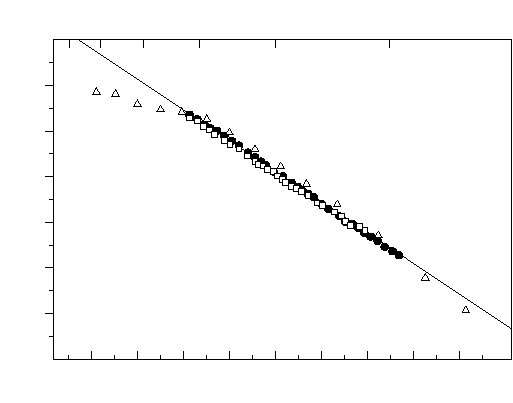
\includegraphics[width=10cm]{../figures/Arrhenius.png}
  \captionof{figure}{`Arrhenius' diagram of three step-heating experiments of
    $^4$He in apatite, showing simple diffusion behaviour in agreement
    with Equation \ref{eq:Arrhenius}. Extrapolating the linear trend
    to geological time scales yields a `closure temperature' of
    $\sim$60$^\circ$C (Equation \ref{eq:Tc}). Modified from
    \citet{braun2006}.}
  \label{fig:Arrhenius}
\fi

\section{Fission tracks}
\label{sec:fission-tracks}

In addition to $\alpha$, $\beta$ and $\gamma$ decay, which form the
basis of the U-Th-Pb (Section \ref{sec:U-Pb}) and U-Th-He (Section
\ref{sec:U-Th-He}) methods, a tiny fraction (1/1,000,000) of the
$^{238}$U atoms decay by \emph{spontaneous fission} (Section
\ref{sec:radioactivity}). In this decay mechanism, the parent nuclide
(i.e., $^{238}$U) decays into two daughter nuclides of roughly equal
mass (e.g., Ba and Kr). These two particles carry a large amount of
energy ($\sim$ 170 MeV) and, having a positive charge, strongly repel
each other. Each of the two fission fragments travels through the
crystal lattice of the host mineral, leaving a trail of damage
behind. Although fission tracks can be directly observed by
transmission electron microscopy (TEM), a more practical approach is
to etch (a polished surface of) the host mineral with acid. This
enlarges the damage zones and makes it possible to count them under an
ordinary petrographic microscope. The volume density $n_s$ (in
cm$^{-3}$) of the fission tracks is given by:
\begin{equation}
n_{s} = \frac{\lambda_f}{\lambda} [^{238}U] \left(e^{\lambda t}-1\right)
\label{eq:Ns}
\end{equation}

where $[^{238}U]$ stands for the volume density the $^{238}$U atoms,
$\lambda_f$ is the fission decay constant
($8.46\times{10}^{-17}$ yr$^{-1}$) and $\lambda$ is the total decay
constant of $^{238}$U ($1.55125\times{10}^{-10}$yr$^{-1}$, see Section
\ref{sec:U-Pb}). The (unobservable) volume density of the tracks is
related to the (observable) surface density $\rho_s$ (in cm$^{-2}$)
by:
\begin{equation}
\rho_s = g_s L n_s
\label{eq:rhos}
\end{equation}

Where g\textsubscript{s} is geometry factor (g\textsubscript{s}=1 if
determined on an internal and g\textsubscript{s}=1/2 on an external
surface) and L is the etchable length of a fission track
($\sim$15$\mu$m). Rearranging Equation \ref{eq:Ns} for time:
\begin{equation}
t = \frac{1}{\lambda}
\ln\left(\frac{\lambda}{\lambda_f}\frac{\rho_s}{[^{238}U] g_s L
}+1\right)
\label{eq:tFT}
\end{equation}

In practice, $[^{238}U]$ is determined by irradiating the (etched)
sample with thermal neutrons in a reactor. This irradiation induces
synthetic fission of $^{235}$U in the mineral (Equation
\ref{eq:235Ufission}). These tracks can be monitored by attaching a
mica detector to the polished mineral surface and etching this monitor
subsequent to irradiation (Figure \ref{fig:EDM}). The surface density
of the induced tracks in the mica detector ($\rho_i$) is a function of
the nuclear cross section of the neutron-induced fission reaction on
$^{235}$U and the neutron fluence in the reactor, both of which are
unknown. A pragmatic solution to this problem is found by irradiating
the sample along with a standard of known age, and lumping all the
unknown parameters together into a calibration factor ($\zeta$), so
that the age of the sample reduces to:
\begin{equation}
t =
\frac{1}{\lambda}\ln\left(1+\frac{g_i}{g_s}\lambda\zeta\rho_d\frac{\rho_s}{\rho_i}\right)
\label{eq:tzeta}
\end{equation}

where $g_s$ = 1, $g_i$ = 1/2 and $\rho_d$ is the surface density of
the induced fission tracks in a dosimeter glass of known (and
constant) U concentration. The latter value is needed to `recycle' the
$\zeta$ value from one irradiation batch to the next, as neutron
fluences might vary through time, or within a sample stack.\\

\ifpdf
\ifuclnotes
\begin{figure}[!ht]
  \centering
  \def\svgwidth{.8\textwidth}
  \input{EDM.pdf_tex}
  \caption{Schematic diagram illustrating the external detector method
    for fission track geochronology \citep[modified
      from][]{galbraith2005}.}
  \label{fig:EDM}
\end{figure}
\else % end of uclnotes
\begin{figure}[!ht]
\noindent\begin{minipage}[t]{.6\textwidth}
\strut\vspace*{-\baselineskip}\newline
\def\svgwidth{\textwidth}
\input{EDM.pdf_tex}
\end{minipage}
\begin{minipage}[t]{.4\textwidth}
  \captionof{figure}{Schematic diagram illustrating the external
    detector method for fission track geochronology \citep[modified
      from][]{galbraith2005}.}
  \label{fig:EDM}
\end{minipage}
\end{figure}
\fi % end of pdf
\else
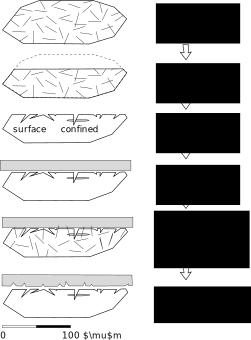
\includegraphics[width=10cm]{../figures/EDM.png}
\caption{Schematic diagram illustrating the external detector method
  for fission track geochronology \citep[modified
    from][]{galbraith2005}.}
  \label{fig:EDM}
\fi

Laboratory experiments have revealed that fission tracks are sensitive
to heat.  For example, it suffices that apatite is heated to
500$^{\circ}$C for 1 hour for all the latent fission tracks to
anneal. Moderate heating shortens the tracks and reduces their surface
density and, hence, the apparent age of the sample. In boreholes, the
apparent fission track age remains constant until a depth is reached
where the ambient temperature is high enough for the tracks to be
reduced in size and number.  This region is called the \emph{Partial
  Annealing Zone} (PAZ). Below the PAZ, no tracks are retained (Figure
\ref{fig:stockli}). The reduction of the surface density of the
spontaneous tracks per unit time can be written as a function of
temperature (T, in Kelvin):

\begin{equation}
\frac{d\rho_s}{dt} = -C \rho_s e^{-E_a/kT}
\label{eq:trackArrhenius}
\end{equation}

where C is a material constant, $E_a$ is the activation energy for
track shortening and k is the Boltzmann constant
(8.616$\times$10$^{-5}$eV/K). Integration of Equation
\ref{eq:trackArrhenius} yields:

\begin{equation}
\ln\left(\frac{\rho_\circ}{\rho}\right) = C~t~e^{-E_a/kT}
\label{eq:lnrho0rho}
\end{equation}

where $\rho_\circ$ is the initial track density prior to
heating. Taking logarithms:

\begin{equation}
\ln(t) = \frac{E_A}{kT} + \ln\left[\ln\left(\frac{\rho_\circ}{\rho}\right)\right] - \ln(C)
\label{eq:lnt}
\end{equation}

For any given \emph{retention coefficient} $\rho_\circ/\rho$, there
exists a linear relationship between ln(t) and 1/T. This is an
\emph{Arrhenius trend} similar to the one described by Equation
\ref{eq:Arrhenius} in the context of U-Th-He thermochronology.  By
extrapolating the Arrhenius diagram to long time scales
($t\sim10^6$yr), it is possible to calculate a `closure temperature'
$T_c$ similar to that which is calculated for the U-Th-He system. For
apatite, T$_c \approx 100^{\circ}C$, whereas for zircon, T$_c \approx
240^{\circ}C$.\\

If a sample has spent some of its time inside the PAZ, then the
subpopulation of its fission tracks formed during that thime will be
shorter than those that subsequently formed above the PAZ. The
probability distribution of the fission track lengths can be
determined by measuring the distance between the two tips of a large
number of (100, say) \emph{horizontally confined} fission tracks under
the optical microscope.  Sophisticated inverse modelling algorithms
have been developed to interpret these length distributions and
extract continuous time-temperature (t-T) paths from them. Such
modelling exercises have become an integral part of modern fission
track studies.

\begin{figure}[!ht]
  \centering
  \ifpdf
  \ifuclnotes
  \def\svgwidth{.9\textwidth}
  \else
  \def\svgwidth{.7\textwidth}
  \fi
  \input{stockli.pdf_tex}
  \else
  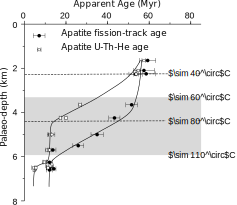
\includegraphics[width=10cm]{../figures/stockli.png}
  \fi
  \caption{Vertical profile of U-Th-He and fission track ages in
    apatite, collected along the footwall of an exhumed normal fault
    block in the White Mountains of eastern California. Samples at the
    highest elevations have resided at shallow depths for up to 55
    Myr. Dashed lines show the extent of the `Partial Retention Zone'
    (PRZ), in which apatite has partially lost its radiogenic
    helium. The grey area indicates the `Partial Annealing Zone',
    where fission tracks have been shortened. At low elevations, young
    ages are observed, indicating rapid exhumation by the normal fault
    at 12 Ma. Additionally, the U-Th-He data show a hint of a second
    exhumation phase at 5 Ma (modified from Stockli, Farley and
    Dumitru, 2000, \textit{Geology} v. 28, no. 11, p. 983-986).}
  \label{fig:stockli}
\end{figure}


\chapter[Cosmogenic Nuclides]{Cosmogenic nuclide geochronology}
\label{sec:cosmo}

The Earth is constantly bombarded by galactic cosmic rays, which
primarily consist of protons. Many of these electrically charged
particles never reach our planet because they are deflected back into
space by the Earth's magnetic field (see Equation \ref{eq:Hev}). The
degree of `protection' provided by the magnetic field is greater at
low latitudes (where the magnetic field lines run parallel to the
surface) than at the poles (where they are perpendicular to the
surface). Thus, the cosmic ray intensity at the equator is
significantly lower than at the poles, although the average energy (or
`rigidity') of the cosmic rays is higher\footnote{At the poles, even
  low energy solar cosmic rays (which predominantly consist of
  electrons, not protons) can reach the upper atmosphere, giving rise
  to the Aurora Borealis.}\\

The primary cosmic rays which do manage to pass through the magnetic
field strongly interact with the atmosphere and form a secondary
cosmic ray `shower', which is mostly made of neutrons and muons. This
secondary cosmic ray shower is rapidly attenuated as it travels down
into the atmosphere. Only a very small fraction of the secondary
cosmic rays, which mostly consist of neutrons, reach the surface of
the Earth. These neutrons then collide with the elements that are
found in rocks and soils, such as silicon, oxygen, calcium etc. When
such an element is hit by a cosmic ray, it undergoes `spallation',
which basically means that it explodes into smaller particles. Most of
these particles are either very short lived or very common in the
Earth's crust. But some of the spallation products are very rare yet
sufficiently long lived to accumulate in measurable quantities in
terrestrial rocks. One example is $^{10}$Be, which has a half life of
1.3 million years. This is orders of magnitude shorter than the age of
the Earth. So, just like the $^{14}$C discussed in Section
\ref{sec:14C}, the existence of $^{10}$Be on our planet would be
impossible to explain without these cosmogenic production pathways. \\

The production of \emph{cosmogenic nuclides} is restricted to the
uppermost few meters below the surface. So if the concentration of the
$^{10}$Be in the surface rocks is known, and if the production rate is
known, then the exposure age of the rock can be estimated. This is
similar to measuring how long a person has been exposed to sunlight by
measuring the tan of their skin. During the 20 years or so that
cosmogenic nuclide geochronology has been around, it has truly
revolutionised various aspects of geomorphology, such as the study of
volcanoes, river incision, landslides, glaciers, sediments, and
faults.\\

\begin{table}[!ht]
\centering
\begin{tabular}{l@{~}l@{~}l@{~}l}
nuclide & half life & reaction types & target minerals \\
\hline
$^3$He & stable & spallation on O, Si & olivine, pyroxene \\
$^{21}$Ne & stable & spallation on Mg, Fe & quartz \\
$^{10}$Be & 1.36 Myr & $^{16}$O(n,4p3n)$^{10}$Be & quartz \\
~ & ~ & $^{28}$Si(n,x)$^{10}$Be & ~ \\
$^{26}$Al & 717 kyr & $^{28}$Si(n,p2n)$^{26}$Al & quartz\\
$^{36}$Cl & 301 kyr & $^{40}$Ca(n,2n3p)$^{36}$Cl & calcite, plagioclase\\
~ & ~ & $^{39}$K($\mu^-$,p2n)$^{36}$Cl & ~ \\
~ & ~ & $^{40}$Ca($\mu^-$,$\alpha$)$^{36}$Cl & ~ \\
~ & ~ & $^{35}$Cl(n,$\mu$)$^{36}$Cl & ~ \\
$^{14}$C & 5730 yr & $^{16}$O(n,2pn)$^{14}$C & quartz\\
\end{tabular}
\caption{Commonly used terrestrial cosmogenic nuclides.}
\label{tab:cosmo}
\end{table}

Table \ref{tab:cosmo} lists the most commonly used cosmogenic
nuclides. What all these isotopes have in common is that they are
normally absent from rocks that are shielded from cosmic rays. They
belong to two categories. There are the cosmogenic noble gases, which
are stable, and the cosmogenic radionuclides, which are
radioactive. Each of these have different applications.

\section{Stable nuclides}

In the simplest case of a stable nuclide in the absence of erosion,
its concentration increases linearly with time (t). So if we measure
the concentration (N) in atoms per gram of, say, quartz, and if we
know the production rate (P), in atoms per gram per year, then we can
simply calculate the age by dividing the concentration by the
production rate:

\begin{equation}
t = \frac{N}{P}
\label{eq:cosmo-exposure}
\end{equation}

Next, consider the situation of a stable nuclide and a rock surface
that is in steady state erosion. To understand this situation, it is
useful to imagine one in the place of a rock particle under an eroding
surface. As the particle approaches the surface, it sees an
exponentially increasing cosmic ray intensity and cosmogenic nuclide
production rate. So in the case of an eroding surface, the cosmogenic
nuclide content can be used not to measure an exposure age, but an
erosion rate ($\epsilon$). $\epsilon$ is a simple function of the
production rate $P$ and the concentration $N$, multiplied by a factor
$\Lambda/\rho$, where $\rho$ is the rock density and $\Lambda$ is the
attenuation length ($\sim$160 g/cm$^{-2}$).  This factor quantifies
how rapidly the cosmic ray intensity decreases with depth in the rock:

\begin{equation}
\epsilon = \frac{\Lambda}{\rho} \frac{P}{N}
\label{eq:cosmo-erosion}
\end{equation}

\section{Radionuclides}

Let us now move on to a cosmogenic radionuclide in a surface that
undergoes no erosion. Initially, the concentration of the nuclide
increases almost linearly with time, but after a while, some of these
nuclides are lost due to radioactive decay. Eventually, after five or
so half lives, a saturation point is reached at which the production
rate is balanced by the decay rate. This provides a hard upper limit
of the exposure ages that can be measured with cosmogenic
radionuclides. The age equation is again a function of $P$ and $N$,
but with the addition of a logarithm and the radioactive decay
constant $\lambda$:

\begin{equation}
t = -\frac{1}{\lambda} \ln\left(1-\frac{N\lambda}{P}\right)
\label{eq:cosmo-radioexposure}
\end{equation}

Finally, here is the full ingrowth equation in the general case of a
cosmogenic radionuclide with a finite exposure age that also undergoes
erosion:

\begin{equation}
N = \frac{P}{\lambda + \rho\epsilon/\Lambda}
\left(1-e^{-(\lambda+\rho\epsilon/\Lambda)t}\right) e^{-\lambda\tau}
\label{eq:cosmo-N}
\end{equation}

with:\\

$N$ = concentration (at/g)\\
\indent $P$ = production rate (at/g/yr)\\
\indent $\lambda$ = decay constant (yr$^{-1}$)\\
\indent $\Lambda$ = attenuation length (g/cm$^{-2}$)\\
\indent $\rho$ = density (g/cm$^{-3}$)\\
\indent $\epsilon$ = erosion rate (cm/yr)\\
\indent $t$ = exposure age (yr)\\
\indent $\tau$ = burial age (yr)\\

There is one additional parameter, $\tau$, which is the \emph{burial
  age}, which will be discussed in Section \ref{sec:banana}. The
important thing to note here is that there is one equation but three
unknowns, the exposure age $t$, the erosion rate $\epsilon$, and the
burial age $\tau$. So in order to solve this equation, two assumptions
are needed. For example, if we assume zero burial ($\tau$ = 0) and
zero erosion ($\epsilon$ = 0), then we calculate the exposure age
($t$). Alternatively, we can assume zero burial and an infinite
exposure age ($\tau$ = 0, t=$\infty$) and calculate the steady state
erosion rate ($\epsilon$). The only way to avoid making such
assumptions and simultaneously determining both the erosion rate and
the exposure age is to measure two nuclides with different half
lives. The most common examples of such paired measurements are
$^{10}$Be/$^{26}$Al and $^{10}$Be/$^{21}$Ne. A convenient method to
plot and interpret such datasets is the two nuclide diagram or `banana
plot'.

\section{The `Banana Plot'}
\label{sec:banana}

When we plot the $^{26}$Al/$^{10}$Be-ratio against the $^{10}$Be
concentration, we obtain the diagram shown in Figure \ref{fig:banana}.
Each part of this diagram has its own applications, which will be
briefly summarised next.\\

\begin{figure}[!ht]
  \centering
  \ifpdf
  \def\svgwidth{.8\textwidth}
  ~~(i)~\input{AlBe.pdf_tex}\\
  \def\svgwidth{.8\textwidth}
  (ii)\input{NeBe.pdf_tex}
  \else
  (i)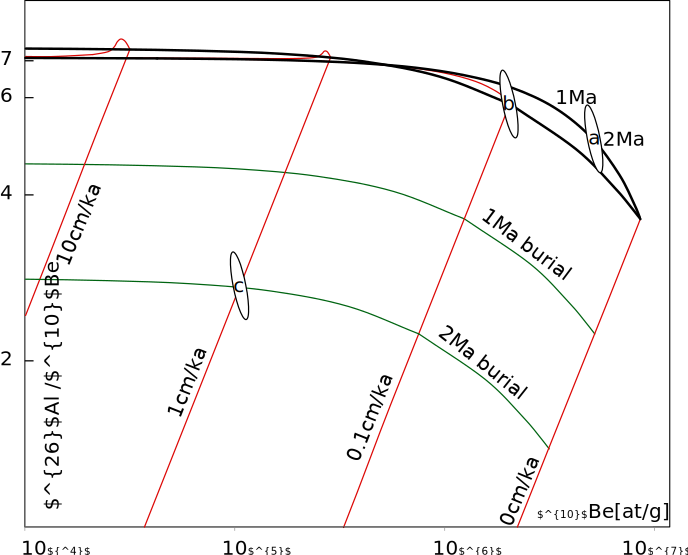
\includegraphics[width=5cm]{../figures/AlBe.png}
  (ii)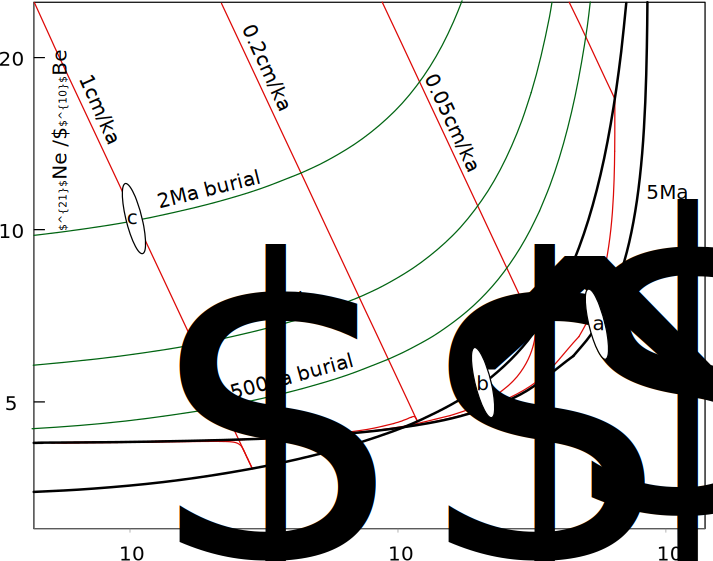
\includegraphics[width=5cm]{../figures/NeBe.png}
  \fi
  \caption{$^{10}$Be/$^{26}$Al (i) and $^{21}$Ne/$^{10}$Be (ii) two
    nuclide (`banana') plots. Sample a has undergone a simple exposure
    history with $t$ = 2Ma, $\epsilon = 0$ and $\tau$ = 0, sample b has
    undergone steady-state erosion at $\epsilon$ = 0.1cm/kyr (t =
    $\infty$ and $\tau$ = 0), whereas sample c has experience a complex
    exposure history. Assuming steady-state erosion prior to burial, the
    data are compatible with $\epsilon$ = 1 cm/kyr followed by 2 Myr of
    burial. The ellipses mark the 95\% confidence bounds for the
    analytical uncertainties (see Section \ref{ch:error-propagation}).}
  \label{fig:banana}
\end{figure}

First consider a sample that plots on the upper line of the
diagram. This is the so-called \emph{zero erosion line}, which groups
all samples that can be used for proper exposure dating. So if a
sample plots on this line, we have effectively verified the assumption
that $\epsilon=0$.  The most important example of studies which
require samples that plot on the zero erosion line are exposure dating
studies of glacial retreat. When glacial striations can be observed on
rock surfaces, this indicates that erosion has been negligible. All
those surfaces should plot on the zero erosion line of the banana
plot.\\

The next line down groups all the samples that are in an erosional
steady state and that, in principle have an infinite exposure age
($t=\infty$), which effectively means an exposure age that is greater
than five times the half lives of both nuclides.  Although erosion
studies can be performed in bedrock, they are actually most commonly
done on sediments. The motivation for this is as follows. Consider a
landscape that is in an erosional steady state and that is irradiated
by cosmic rays. Cosmogenic nuclides such as $^{10}$Be accumulate in
the first 2m or so below the surface. These rocks are removed and
transported down the drainage network, carrying the cosmogenic nuclide
signal with them. By measuring the $^{10}$Be content of a single
sample of river sediment, the average erosion rate of the entire
catchment can be calculated.\\

So the upper line of the $^{10}$Be/$^{26}$Al banana plot is the zero
erosion line, the lower line is the steady state erosion line, and the
area between them is called the \emph{steady state erosion island} (or
\emph{banana}).  Above the erosion island is the `forbidden zone' of
physically impossible cosmogenic nuclide compositions. Samples
plotting in this area are likely to suffer from methodological or
analytical errors. The large area below the erosion island is the zone
of \emph{complex exposure histories}, in which we can find samples
that have undergone at least one phase of burial. For example,
consider a river sediment derived from a catchment that is in an
erosional steady state (e.g., $\epsilon$ = 0.1cm/kyr) and has
accumulated a measurable amount of cosmogenic $^{10}$Be and
$^{26}$Al. Suppose that this sediment is washed into a cave.  The roof
of the cave will shield the sample from cosmic rays, so that the
production of $^{10}$Be and $^{26}$Al stops, but their radioactive
decay continues. So with time, the sample will move down a line on the
banana plot. The burial age can be calculated from the distance of the
sample below the steady state erosion island.  Obviously, the most
common application of burial dating is the dating of cave
sediments. By measuring the age of different cave levels in the walls
of a river canyon, it is possible to determine the rate of canyon
incision.

\section{Scaling models}
\label{sec:scaling}

So far in this Chapter, we have assumed that the cosmogenic nuclide
production rate $P$ is known. In reality, however, this is only the
case for a handful of locations (`calibration sites') in the world,
where the exposure history of rocks is known through independent means
(e.g. by $^{14}$C dating of organic matter or $^{40}$Ar/$^{39}$Ar
dating of lava flows. These production rates are only valid for the
specific conditions (latitude, elevation, age) of each particular
calibration site. To apply the cosmogenic nuclide method to other
field settings, the production rates must be scaled to a common
reference at sea level and high latitude (SLHL). Up to 20\%
uncertainty is associated with this scaling, constituting the bulk of
cosmogenic nuclide age uncertainty.\\

Although several efforts have been made to directly measure production
rate scaling with latitude and elevation using artificial H$_{2}$O and
SiO$_2$ targets, all currently used scaling models are based on
neutron monitor surveys. The oldest and still most widely used scaling
model is that of Lal (1991). This model is a simple set of polynomial
equations giving the (spallogenic + muogenic) production rate relative
to SLHL as a function of geographic latitude and elevation.\\

Despite their limitations, the production rate scaling factors allow
the calculation of TCN production rates at any location on the Earth's
surface, assuming that the sample is a slab of zero thickness taken
from a horizontal planar surface. If these assumption are not
fulfilled, the SLHL production rates must be multiplied by a second
set of correction factors, quantifying the extent to which the cosmic
rays were blocked by topographic obstructions, snow cover, and the
thickness of the sample (`self shielding').


\chapter[U-series dating]{U-series disequilibrium methods}
\label{ch:intro2Useries}

In Section \ref{sec:decay-series}, we saw that the
$^{235}$U-$^{207}$Pb and $^{238}$U-$^{206}$Pb decay series generally
reach a state of \emph{secular equilibrium}, in which the activity
(expressed in decay events per unit time) of each intermediate
daughter product is the same, so that:

$$D_n \lambda_n = \cdots  = D_2 \lambda_2 = D_1 \lambda_1 = P \lambda_P$$

as described by Equation \ref{eq:NDnLn}. However, certain natural
processes can disturb this equilibrium situation, such as chemical
weathering, precipitation from a solution, (re-)crystallisation
etc. The leads to two new types of chronometric systems:

\begin{enumerate}
\item An intermediate daughter isotope in the decay series is
  separated from its parent nuclide incorporated into a rock or
  sediment, and decays according to its own half life.
\item A parent nuclide has separated itself from its previous decay
  products and it takes some time for secular equilibrium to be
  re-established.
\end{enumerate}

This idea is most frequently applied to the $^{238}$U-decay series,
notably $^{230}$Th and $^{234}$U. The first type of disequilibrium
dating forms the basis of the $^{234}$U-$^{238}$U and $^{230}$Th
methods (Sections \ref{sec:234238} and \ref{sec:230}). The second
forms the basis of the $^{230}$Th-$^{238}$U method (Section
\ref{sec:230238})

\section{The $^{234}$U-$^{238}$U method}
\label{sec:234238}

The activity ratio of $^{238}$U to its third radioactive daughter
$^{234}$U in the world's oceans is $A(^{234}U)/A(^{238}U)$ $\equiv$
$\gamma_\circ$ $\approx$ 1.15. The slight enrichment of the $^{234}$U
over $^{238}$U is attributed to $\alpha$-recoil of its immediate
parent $^{234}$Th and the fact that $^{234}$U is more `loosely bound'
inside the crystal lattice of the host mineral, because it is
preferentially seated in sites which have undergone radiation
damage. Once the oceanic U is incorporated into the crystal structure
of marine carbonates, the radioactive equilibrium gradually restores
itself with time. The total activity of $^{234}$U is made up of a
component which is supported by secular equilibrium (and equals the
activity of $^{238}U$) and an `excess' component, which decays with
time:

\begin{equation}
A(^{234}U) = A(^{238}U) + A(^{234}U)^x_\circ e^{-\lambda_{234}t} 
\label{eq:A234}
\end{equation}

where $A(^{234}U)^x_\circ$ is the initial amount of excess $^{234}$U
and $\lambda_{234}$ = 2.8234 $\times$ 10$^{-6}$ yr$^{-1}$ (t$_{1/2}$ =
245.5 kyr). Let $A(^{234}U)_\circ$ be the initial total $^{234}$U
activity. Then:

\begin{equation}
A(^{234}U) = A(^{238}U) + \left[A(^{234}U)_\circ - A(^{238}U) \right] e^{-\lambda_{234}t} 
\label{eq:A234b}
\end{equation}

Dividing by A($^{238}$U):

\begin{equation}
\frac{A(^{234}U)}{A(^{238}U)} = 1 + [ \gamma_\circ - 1 ] e^{-\lambda_{234}t} 
\label{eq:A234A238}
\end{equation}

Which can be solved for $t$ until about 1 Ma.

\section{The $^{230}$Th method}
\label{sec:230}

U and Th are strongly incompatible elements. This causes chemical
fractionation and disturbs the secular equilibrium of the $^{238}$U
decay series in young volcanic rocks. It is commonly found that the
activity ratio $A(^{230}Th)/A(^{238}U)$ $>$ 1. As expected, the
secular equilibrium between $^{234}$U and $^{238}$U is not disturbed
by chemical fractionation, so that $A(^{234}U)/A(^{238}U)$ = 1. The
total $^{230}$Th activity is given by:

\begin{equation}
A(^{230}Th) = A(^{230}Th)_\circ^x e^{-\lambda_{230}t} + A(^{238}U)(1-e^{-\lambda_{230}t})
\label{eq:A230}
\end{equation}

where $A(^{230}Th)_\circ^x$ is the initial amount of `excess'
$^{230}$Th at the time of crystallisation and $A(^{238}U)=A(^{234}U)$
due to secular equilibrium of the U isotopes. Thus, the first term of
Equation \ref{eq:A230} increases with time from 0 to A($^{238}$U)
while the second term decreases from $A(^{230}Th)_\circ^x$ to
0. Dividing by $A(^{232}Th)$ yields a linear relationship between
$A(^{230}Th)/A(^{232}Th)$ and $A(^{238}U) / A(^{232}Th)$:

\begin{equation}
\frac{A(^{230}Th)}{A(^{232}Th)} = \frac{A(^{230}Th)_\circ^x}{A(^{232}Th)} e^{-\lambda_{230}t} + 
\frac{A(^{238}U)}{A(^{232}Th)}(1-e^{-\lambda_{230}t})
\label{eq:230232}
\end{equation}

This forms an isochron with slope ($1-e^{-\lambda_{230}t}$), from
which the age $t$ can be calculated. This method is applicable to
volcanic rocks and pelitic ocean sediments ranging from 3ka to 1Ma.

\section{The $^{230}$Th-$^{238}$U method}
\label{sec:230238}

Uranium is significantly more soluble in water than Th. As a result,
the intermediate daughter $^{230}$Th is largely absent from sea
water. Thus, lacustrine and marine carbonate rocks contain some U but
virtually no Th at the time of formation. The $^{230}$Th activity
increases steadily with time as a result of $^{234}$U decay. The total
$^{230}$Th activity consists of a growing component $A(^{230}Th)^s$
that is in secular equilibrium with $^{238}U$ and a shrinking
component $A(^{230}Th)^x$ of `excess' $^{230}$Th produced by the
surplus of $^{234}$U commonly found in ocean water (see section
\ref{sec:234238}):

\begin{align}
~ & A(^{230}Th) =  A(^{230}Th)^s + A(^{230}Th)^x \label{eq:230total}\\
\mbox{with:~} & A(^{230}Th)^s = A(^{238}U) (1-e^{-\lambda_{230}t}) \label{eq:230s}\\
\mbox{and:~} & A(^{230}Th)^x = \frac{\lambda_{230}}{\lambda_{230}-\lambda_{234}} 
A(^{234}U)_\circ^x\left(e^{-\lambda_{234}t}-e^{-\lambda_{230}t}\right) \label{eq:230x}
\end{align}

In which the expression for $A(^{230}Th)^x$ follows from Equation
\ref{eq:ND1} and $A(^{234}U)_\circ^x$ denotes the initial amount of
excess $^{234}$U activity (as in Section \ref{sec:234238}). Taking
into account that $A(^{234}U)_\circ^x = A(^{234}U)_\circ -
A(^{238}U)$, and dividing by $A(^{238}U)$, we obtain:

\begin{equation}
\frac{A(^{230}Th)^x}{A(^{238}U)} = \frac{\lambda_{230}}{\lambda_{230}-\lambda_{234}} (\gamma_\circ-1)
\left(e^{-\lambda_{234}t}-e^{-\lambda_{230}t}\right)
\label{eq:230238x}
\end{equation}

in which $\gamma_\circ \equiv A(^{234}U)/A(^{238}U)$ as defined in
Section \ref{sec:234238}. The formation age of the carbonate can be
calculated by substituting Equations \ref{eq:230s} and \ref{eq:230238x}
into \ref{eq:230total} and solving for $t$. 

\begin{equation}
  \frac{A(^{230}Th)}{A(^{238}U)} = 1 - e^{-\lambda_{230}t} +
  \frac{\lambda_{230}}{\lambda_{230}-\lambda_{234}} (\gamma_\circ-1)
\left(e^{-\lambda_{234}t}-e^{-\lambda_{230}t}\right)
\label{eq:230238}
\end{equation}

If $\gamma_\circ = 1$ (i.e., the water is in secular equilibrium for
U), then Equation \ref{eq:230total} simplifies to:

\begin{equation}
\frac{A(^{230}Th)}{A(^{238}U)} = 1-e^{-\lambda_{230}t}
\label{eq:230238b}
\end{equation}

If $\gamma_\circ \neq 0$, Equation \ref{eq:230238b} yields ages that
are systematically too old, unless $t$ $<$ 100ka and $\gamma_\circ \leq
1.15$.


\chapter{Error propagation}
\label{ch:error-propagation}

All the methods and equations presented thus far have assumed that all
parameters are either known or measured with infinite precision. In
reality, however, the analytical equipment used to measure isotopic
compositions, elemental concentrations and radioactive half-lives is
not perfect.  It is crucially important that we quantify the resulting
analytical uncertainty before we can reliably interpret the resulting
ages.\\

For example, suppose that the extinction of the dinosaurs has been
dated at 65 Ma in one field location, and a meteorite impact has been
dated at 64 Ma elsewhere.  These two numbers are effectively
meaningless in the absence of an estimate of precision. Taken at face
value, the dates imply that the meteorite impact took place 1 million
years after the mass extinction, which rules out a causal relationship
between the two events. If, however, the analytical uncertainty is
significantly greater than 1 Myr (e.g. 64 $\pm$ 2 Ma and 65 $\pm$ 2
Ma), then such of a causal relationship remains very plausible.

\section{Some basic definitions}
\label{sec:summarystatistics}

Suppose that our geochronological age ($t$) is calculated as a function
($f$) of some measurements ($x$ and $y$):

\begin{equation}
t = f(x,y)
\label{eq:tfxy}
\end{equation}

Suppose that we have performed a large number ($n$) of replicate
measurements of $x$ and $y$:

\begin{equation}
\left\{
\begin{array}{rl}
x = & \{x_1, x_2, \cdots, x_i, \cdots, x_n\} \\
y = & \{y_1, y_2, \cdots, y_i, \cdots, y_n\}
\end{array}
\right.
\label{eq:xy}
\end{equation}

It is useful to define the following \emph{summary statistics}:

\begin{enumerate}
\item The mean:
\begin{equation}
\left\{
\begin{array}{rl}
\overline{x} \equiv & \frac{1}{n} \sum_{i=1}^{n} x_i\\
\overline{y} \equiv & \frac{1}{n} \sum_{i=1}^{n} y_i
\end{array}
\right.
\label{eq:mean}
\end{equation}

is a useful definition for the `most representative' value of $x$ and
$y$, which can be plugged into Equation~\ref{eq:tfxy} to calculate the
`most representative' age.

\item The variance:
\begin{equation}
\left\{
\begin{array}{rl}
s[x]^2 \equiv & \frac{1}{n-1} \sum_{i=1}^{n} (x_i-\overline{x})^2\\
s[y]^2 \equiv & \frac{1}{n-1} \sum_{i=1}^{n} (y_i-\overline{y})^2
\end{array}
\right.
\label{eq:variance}
\end{equation}

with $s[x]$ and $s[y]$ the `standard deviations', is used to quantify
the amount of dispersion around the mean.

\item The covariance:
\begin{equation}
s[x,y] \equiv \frac{1}{n-1} \sum_{i=1}^{n} (x_i-\overline{x})(y_i-\overline{y})
\label{eq:covariance}
\end{equation}

quantifies the degree of correlation between variables $x$ and $y$.
\end{enumerate}

$\overline{x}$, $\overline{y}$, $s[x]^2$, $s[y]^2$ and $s[x,y]$ can
all be estimated from the input data $(x,y)$. These values can then be
used to infer $s[t]^2$, the variance of the calculated age $t$, a
process that is known as `error propagation'. To this end, recall the
definition of the variance (Equation \ref{eq:variance}):

\begin{equation}
s[t]^2 \equiv \frac{1}{n-1} \sum_{i=1}^{n} (t_i-\overline{t})^2
\label{eq:vart}
\end{equation}

We can estimate $(t_i-\overline{t})$ by differentiating Equation
\ref{eq:tfxy}:

\begin{equation}
t_i - \overline{t} = (x_i-\overline{x}) \frac{\partial f}{\partial x} +
(y_i-\overline{y}) \frac{\partial f}{\partial y}
\label{eq:ti-t}
\end{equation}

Plugging Equation \ref{eq:ti-t} into \ref{eq:vart}, we obtain:

\begin{align}
s[t]^2 & = \frac{1}{n-1} \sum_{i=1}^{n} \left[
(x_i-\overline{x}) \left(\frac{\partial f}{\partial x}\right) +
(y_i-\overline{y}) \left(\frac{\partial f}{\partial y}\right) \right]^2 \label{eq:s2t1}\\
~ & = s[x]^2 \left(\frac{\partial f}{\partial x}\right)^2 +
s[y]^2 \left(\frac{\partial f}{\partial y}\right)^2 +
2~s[x,y] \frac{\partial f}{\partial x} \frac{\partial f}{\partial y} \label{eq:s2t}
\end{align}

This is the general equation for the propagation of uncertainty with
two variables, which is most easily extended to more than two
variables by reformulating Equation \ref{eq:s2t} into a matrix form:

\begin{equation}
s[t]^2 = 
\left[
\begin{array}{@{}c@{~}c@{}}
\frac{\partial t}{\partial x}&\frac{\partial t}{\partial y}
\end{array}
\right]
\left[
\begin{array}{@{}c@{~}c@{}}
s[x]^2 & s[x,y]\\
s[x,y] & s[y]^2
\end{array}
\right]
\left[
\begin{array}{@{}c@{}}
\frac{\partial t}{\partial x} \\
\frac{\partial t}{\partial y}
\end{array}
\right]
\label{eq:s2tmatrix}
\end{equation}

where the innermost matrix is known as the \emph{variance-covariance}
matrix and the outermost matrix (and its transpose) as the
\emph{Jacobian matrix}.  Let us now apply this equation to some simple
functions.

\section{Examples}

Let $x$ and $y$ indicate measured quantities associated with
analytical uncertainty.  And let $a$ and $b$ be some error free
parameters.

\begin{enumerate}
\item{addition:}
\begin{align}
& t = a x + b y \Rightarrow \frac{\partial t}{\partial x} = a, 
\frac{\partial t}{\partial y} = b \nonumber\\
& \Rightarrow s[t]^2 = a^2 s[x]^2 + b^2 s[y]^2 + 2ab~s[x,y]
\label{eq:addition}
\end{align}

\item{subtraction:}
\begin{equation}
t = a x - b y \Rightarrow
s[t]^2 = a^2 s[y]^2 + b^2 s[y]^2 - 2ab~s[x,y]
\label{eq:subtraction}
\end{equation}

\item{multiplication:}
\begin{align}
& t = a x y \Rightarrow \frac{\partial t}{\partial x} = a y, 
\frac{\partial t}{\partial y} = ax \nonumber\\
& \Rightarrow s[t]^2 = (ay)^2 s[x]^2 + (ax)^2 s[y]^2 + 2a^2 xy~s[x,y] \nonumber\\
& \Rightarrow \left(\frac{s[t]}{t}\right)^2 = \left(\frac{s[x]}{x}\right)^2 + 
  \left(\frac{s[y]}{y}\right)^2 + 2 \frac{s[x,y]}{x y}
\label{eq:multiplication}
\end{align}

\item{division:}
\begin{equation}
t = a \frac{x}{y} \Rightarrow
\left(\frac{s[t]}{t}\right)^2 = \left(\frac{s[x]}{x}\right)^2 + 
  \left(\frac{s[y]}{y}\right)^2 - 2 \frac{s[x,y]}{x y}
\label{eq:division}
\end{equation}

\item{exponentiation:}
\begin{equation}
t = a~e^{bx} \Rightarrow \frac{\partial f}{\partial x} = ab~e^{bx} 
\Rightarrow s[t]^2 = (b t)^2 s[x]^2
\label{eq:exponentiation}
\end{equation}

\item{logarithms:}
\begin{equation}
t = a~\ln(bx) \Rightarrow \frac{\partial f}{\partial x} = \frac{a}{x}
\Rightarrow s[t]^2 = a^2 \left(\frac{s[x]}{x}\right)^2
\label{eq:logarithms}
\end{equation}

\item{power:}
\begin{equation}
  t = a x^b \Rightarrow \frac{\partial f}{\partial x} = b \frac{a
    x^b}{x} \Rightarrow \left(\frac{s[t]}{t}\right)^2 =
  b^2\left(\frac{s[x]}{x}\right)^2
\label{eq:power}
\end{equation}

\end{enumerate}

\section{Accuracy vs. precision}

Recall the definition of the arithmetic mean (Equation \ref{eq:mean}):

$$\overline{x} \equiv \frac{1}{n} \sum_{i=1}^{n} x_i$$

Applying the equation for the error propagation of a sum (Equation
\ref{eq:addition}):

\begin{equation}
s[\overline{x}]^2 = \frac{1}{n} \sum_{i=1}^{n} s[x_i]^2 =
\frac{s[x]^2}{n}
\label{eq:varianceofthemean}
\end{equation}

where we assume that all $n$ measurements were done
\emph{independently}, so that $cov(x_i,x_j)=0 \forall i, j$.  The
standard deviation of the mean is known as the \underline{standard
  error}:

\begin{equation}
s[\overline{x}] = \frac{s[x]}{\sqrt{n}}
\label{eq:standarderror}
\end{equation}

This means that the standard error of the mean monotonically decreases
with the square root of sample size. In other words, we can
arbitrarily increase the \emph{precision} of our analytical data by
acquiring more data. However, it is important to note that the same is
generally not the case for the \emph{accuracy} of those data. The
difference between precision and accuracy is best explained by a darts
board analogy:\\

\noindent
\begin{minipage}{\textwidth}
  \centering
  \ifpdf
  \def\svgwidth{\textwidth}
  \input{bullseye.pdf_tex}
  \else
  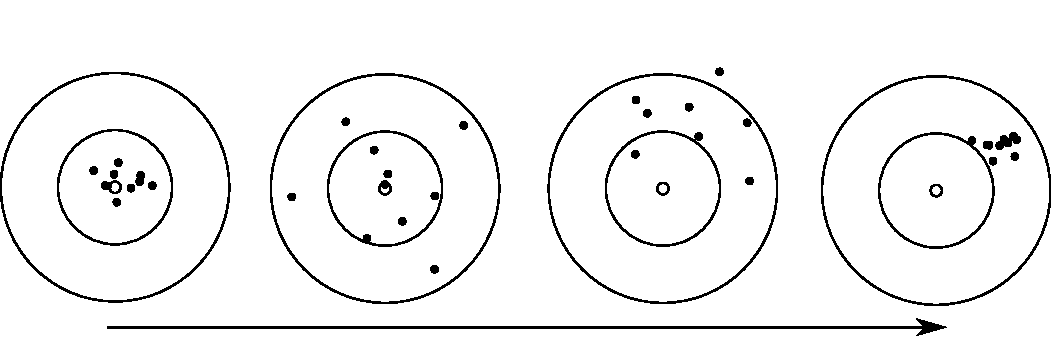
\includegraphics[width=10cm]{../figures/bullseye.png}
  \fi
\end{minipage}

\bigskip

Whereas the analytical precision can be computed from the data using
the error propagation formulas introduced above, the only way to get a
grip on the accuracy is by analysing another sample of independently
determined age. Such test samples are also known as `secondary
standards'.

\ifpdf
\ifuclnotes
\begin{figure}[!ht]
  \centering
  \def\svgwidth{\textwidth}
  \input{covariance.pdf_tex}
  \caption{Four datasets of 100 random numbers (black dots) which have
    the same means (white squares) but different (co-)variance
    structures. The marginal distributions of the $x$ and $y$ variables
    are shown as `bell curves' on the top and right axis of each
    plot.}
  \label{fig:covariance}
\end{figure}
\else % end of uclnotes
\begin{figure}[!ht]
  \noindent\begin{minipage}[t]{.69\textwidth}
\strut\vspace*{-\baselineskip}\newline
\def\svgwidth{\textwidth}
\input{covariance.pdf_tex}
\end{minipage}
\begin{minipage}[t]{.3\textwidth}
  \captionof{figure}{Four datasets of 100 random numbers (black dots) which have
    the same means (white squares) but different (co-)variance
    structures. The marginal distributions of the $x$ and $y$ variables
    are shown as `bell curves' on the top and right axis of each
    plot.}
  \label{fig:covariance}
\end{minipage}
\end{figure}
\fi % end of pdf
\else
\includegraphics[width=10cm]{../figures/covariance.png}
  \captionof{figure}{Four datasets of 100 random numbers (black dots) which have
    the same means (white squares) but different (co-)variance
    structures. The marginal distributions of the $x$ and $y$ variables
    are shown as `bell curves' on the top and right axis of each
    plot.}
  \label{fig:covariance}
\fi


\chapter{Exercises}
\label{sec:exercises}

\begin{enumerate}

\item If helium ions (mass number = 4) are accelerated with a voltage
  of 10 kV in a mass spectrometer, at what speed are they emitted from
  the source? Recall that 1 atomic mass unit (amu) = 1.66 $\times$
  10$^{-27}$ kg and the elementary charge is 1.602 $\times$ 10$^{-19}$
  C. \rotatebox[origin=c]{180}{[Answer: 695 km/s]}

\item We are trying to estimate the Rb concentration in a rock for the
  purpose of whole rock Rb-Sr dating. To this end, we use a spike with
  a Rb concentration of 7.5 ppm containing 99.4\% $^{87}$Rb and 0.6\%
  $^{85}$Rb (these are atomic abundances). We mix 3.5g of the spike
  with 0.25g of sample dissolved in 50g. The $^{87}$Rb/$^{85}$Rb-ratio
  of the mixture is 1.55, as measured by mass spectrometry. What is
  the Rb concentration in ppm? Note that natural Rb comprises of
  27.825\% $^{87}$Rb and 72.165\% $^{85}$Rb.  
  \rotatebox[origin=c]{180}{[Answer: 120 ppm]}

\item A biotite contains 465ppm Rb and 30ppm Sr with a
  $^{87}$Sr/$^{86}$Sr-ratio of 2.50.  Given an initial
  $^{87}$Sr/$^{86}$Sr-ratio of 0.7035, what is the age of the biotite?
  Natural Rb has an atomic mass of 85.4678 and comprises 72.165\%
  $^{85}$Rb and 27.825\% $^{87}$Rb, which has a half life of t$_{1/2}$
  = 48.8 Gyr. Sr has an atomic mass of 87.62. Its non-radiogenic
  isotopes occur with the following abundances: $^{84}$Sr/$^{86}$Sr =
  0.056584 and $^{86}$Sr/$^{88}$Sr = 0.1194.
  \rotatebox[origin=c]{180}{[Answer: 2.36 Ga]}

\item Consider a zircon with the following composition: U = 792.1 ppm,
  Th = 318.6 ppm, Pb = 208.2 ppm. Atomic masses for U, Th and Pb in
  the zircon are 238.04, 232.04 and 205.94, respectively. The isotopic
  composition of the Pb is as follows: $^{204}$Pb = 0.048\%,
  $^{206}$Pb = 80.33\%, $^{207}$Pb = 9.00\%, $^{208}$Pb =
  10.63\%. Assume the following initial Pb composition: 204 : 206 :
  207 : 208 = 1.00 : 16.25 : 15.51 : 35.73. The decay constants for
  $^{238}$U, $^{235}$U and $^{232}$Th are given in Section
  \ref{sec:U-Pb}. $^{238}$U/$^{235}$U = 137.818. Calculate the
  $^{206}$Pb/$^{238}$U, $^{207}$Pb/$^{235}$U, $^{208}$Pb/$^{232}$Th
  and $^{207}$Pb/$^{206}$Pb-age of the zircon. Give an account of its
  formation history. \\ \rotatebox[origin=c]{180}{[Answer: 1.405,
      1.523, 1.284 and 1.689 Ga]}

\item A biotite was separated from granite and dated with the K-Ar
  method. The analytical data are as follows: K$_2$O = 8.45 weight \%,
  radiogenic $^{40}$Ar = 6.015 $\times$ 10$^{-10}$ mol/g.  What is the
  K-Ar age of the biotite? The atomic mass of K is 39.098 (and oxygen
  15.9994), with an isotopic composition that comprises 93.258\%
  $^{39}$K, 6.730\% $^{41}$K and 0.01167\% $^{40}$K, which has a
  half-life of t$_{1/2}$ = 1.248 Gyr. Recall that only 10.72\% of the
  $^{40}$K decays to $^{40}$Ar, with the remaining 89.28\% turning
  into $^{40}$Ca. \rotatebox[origin=c]{180}{[Answer: 47.7 Ma]}

\item Consider a biotite with a conventional K-Ar age of 384Ma. A
  $^{40}$Ar/$^{39}$Ar step-heating experiment yields the following
  data:

\begin{centering}
\begin{tabular}{c@{~}|@{~}c@{~}c@{~}c@{~}c@{~}c@{~}c@{~}c}
\% $^{39}$Ar released & 7 & 15 & 20 & 25 & 35 & 70 & 100\\
$^{40}$Ar$^*/^{39}$Ar & 2.27 & 4.97 & 6.68 & 9.58 & 10.25 & 10.10 & 10.26 \\
\end{tabular}
\end{centering}

The analysis was done using a co-irradiated 1.062 Ga biotite age
standard yielding a $^{40}$Ar$^*$/$^{39}$Ar-ratio of 27.64.  Construct
the $^{40}$Ar/$^{39}$Ar age spectrum and use this to comment on the
thermal history of the host rock. t$_{1/2}$($^{40}$Ar) = 1.248
Gyr.\\ \rotatebox[origin=c]{180}{[Answer: 115, 243, 319, 442, 470, 463
    and 470 Ma]}

\item How many cm$^3$ of helium does a rock weighing 1 kg and
  containing 2 ppm of uranium (but no thorium) produce after 1 billion
  years? The molar volume of an ideal gas is 22.414 litres. Uranium
  has an atomic mass of 238.04 with $^{238}$U/$^{235}$U =
  137.818. Decay constants of U are given in Section \ref{sec:U-Pb}.
  \rotatebox[origin=c]{180}{[Answer: 0.27 cm$^3$]}

\item Repeated analysis of the Fish Canyon zircon age standard (t=27.8
  Ma) yields the following fission track data:
  
\begin{centering}
\begin{tabular}{ccc}
$\rho_s$ & $\rho_i$ & $\rho_d$ \\
($\times$10$^5$cm$^{-2}$) & ($\times$10$^6$cm$^{-2}$) & ($\times$10$^5$cm$^{-2}$)\\
\hline
36.56 & 6.282 & 2.829 \\
38.97 & 7.413 & 3.313 \\
56.53 & 7.878 & 2.457 \\
41.05 & 8.578 & 3.485 \\
45.87 & 6.985 & 2.482
\end{tabular}
\end{centering}

Compute the average $\zeta$-calibration factor and use this to
calculate the zircon fission track ages of the following rocks:

\begin{centering}
\begin{tabular}{r@{~}c@{~}c@{~}c}
~ & $\rho_s$ & $\rho_i$ & $\rho_d$ \\
~ & ($\times$10$^5$cm$^{-2}$) & ($\times$10$^6$cm$^{-2}$) & ($\times$10$^5$cm$^{-2}$)\\
\hline
Tardree rhyolite & 60.49 & 2.66 & 1.519 \\
Bishop tuff & 6.248 & 1.299 & 0.081 \\
\end{tabular}
\end{centering}

The half-life of $^{238}$U is t$_{1/2}$ = 4.47 Gyr.\\
\rotatebox[origin=c]{180}{[Answer: Tardree -- 57 Ma; Bishop -- 643 ka]}

\item The Dry Valleys of Antarctica represent one of the oldest
  landscapes in the world, with erosion rates as low as 2.5
  cm/Myr. Cosmogenic $^{21}$Ne and $^{10}$Be accumulate in quartz at
  SLHL production rates of 20 at/g/yr and 4.5 at/g/yr,
  respectively. What is the expected $^{21}$Ne/$^{10}$Be-ratio in
  these surface rocks? The rock density is 2.65 g/cm$^{3}$ and the
  half-life of $^{10}$Be is 1.36 Myr. The attenuation length for
  cosmic ray neutrons is $\Lambda$=160
  g/cm$^{-2}$. \rotatebox[origin=c]{180}{[Answer: 59.1]}

\item A fossil mollusc has been found in a Quaternary beach formation
  and its activity ratio measured as A($^{230}$Th) / A($^{238}$U) =
  0.6782. Determine the age of the fossil assuming that $\gamma_\circ$
  = 1.15 and given that the half lives of $^{230}$Th and $^{234}$U are
  75,380 and 245,500 years,
  respectively. \rotatebox[origin=c]{180}{[Answer: 100kyr]}

\end{enumerate}


\chapter{Programming practicals}
\label{sec:programming}

In this Chapter you will process some real geochronological datasets
using either \texttt{R} or \texttt{Matlab}. These are both
mathematical scripting languages that are both powerful and easy to
use.\\

\texttt{R} is a free and open programming language that works on any
operating system, including \texttt{Windows}, \texttt{OS-X} and
\texttt{Unix/Linux}. It can be downloaded and installed from
\texttt{http://r-project.org}.\\

\texttt{Matlab} is a proprietary programming environment. The full
version of this software is very expensive but a reasonably complete
student version can be purchased for $\pounds$55 + VAT from
\texttt{http://mathworks.com}. Alternatively, \texttt{Octave} is an
open source clone of \texttt{Matlab} that can be downloaded for free
from \texttt{http://www.gnu.org/software/octave}.\\

Sections~\ref{sec:R} and \ref{sec:Matlab} will present two brief
tutorials of \texttt{R} and \texttt{Matlab}, respectively.  These will
cover most commands that you will need for the subsequent computer
practicals.


\section{Introduction to \texttt{R}}
\label{sec:R}

A number of different graphical user interfaces (GUIs) are available
to interact with \texttt{R}. The most popular of these are
\texttt{Rgui}, \texttt{RStudio}, \texttt{RCommander} and
\texttt{Tinn-R}.

\begin{enumerate}
  \item Starting these applications or running \texttt{R} in a text
    terminal presents the user with a command line prompt. Anything
    that is typed after the \texttt{>} symbol will be evaluated
    immediately. Thus, we can use \texttt{R} as a calculator:

\begin{verbatim}
> 1 + 1
> sqrt(2)
> exp(log(10))
> 31 %% 14
\end{verbatim}

\item Alternatively, code can also be saved as text (using a built-in text
  editor) and saved as \texttt{mycode.R}, say. This code can then be
  copied and pasted at the command line prompt. Or it can be called from
  the command line using the \texttt{source()} function:

\begin{verbatim}
> source('mycode.R')
\end{verbatim}

\item In the remainder of this tutorial, we will assume that your code is
  run from a text file unless explicitly stated otherwise. The
  \texttt{\#}~symbol marks the beginning of a comment.  \texttt{R}
  ignores anything that follows it:

\begin{verbatim}
# The arrow symbol is used to assign a value to a
# variable. Note that the arrow can point both ways:
foo <- 2
4 -> bar
print(foo*bar)

# Defining a vector of multiple values:
myvec <- c(0,1,2,3,4,5)
# or, equivalently:
myvec <- seq(0,5)
# or
myvec <- seq(from=0,to=5,by=1)
# or
myvec <- 0:5

# Turn myvec into a 2x3 matrix:
mymat <- matrix(myvec,nrow=2)

# Accessing one or more elements from a vector or matrix:
x <- myvec[3]
y <- myvec[1:3]
z <- mymat[1,2:3]

# Change the third value in the second row of mymat to 10:
mymat[2,3] <- 10

# Change the entire second column of mymat to -1:
mymat[,2] <- -1

# Transpose of a matrix:
flipped <- t(mymat)

# Element-wise multiplication (*) 
# vs. matrix multiplication (%*%):
rectangle <- mymat * mymat
square <- mymat %*% flipped
\end{verbatim}

\item Lists are used to store more complex data objects:

\begin{verbatim}
mylist <- list(v=myvec,m=mymat,nine=9)
\end{verbatim}

The three components of \texttt{mylist} can be accessed in a number of
equivalent ways. For example, the first item (\texttt{v}) of
\texttt{mylist} can be accessed either as \verb|mylist$v|, as
\verb|mylist[[1]]| or as \verb|mylist[['v']]|.\\

Data frames are list-like tables:

\begin{verbatim}
myframe <- data.frame(period=c('Cz','Mz','Pz','PC'),
                      SrSr=c(0.708,0.707,0.709,0.708),
                      fossils=c(TRUE,TRUE,TRUE,FALSE))
\end{verbatim}

You can access the items in the data frame \texttt{myframe} either
like a list (e.g. \verb|myframe$period|) or like a matrix
(\verb|myframe[,'period']|):

\item If you want to learn more about a function, type \texttt{help()} or
\texttt{?} at the command line prompt:

\begin{verbatim}
> help(c)
> ?matrix
\end{verbatim}

\item In addition to \texttt{R}'s built-in functions, you can also define
  your own:

\begin{verbatim}
cube <- function(n){
    return(n^3)
}

# Using this function to take the cube of 3:
c3 <- cube(3)

# Conditional statement:
toss <- function(){
    if (runif(1)>0.5){ # runif(n) draws n random 
        print("head")  # numbers between 0 and 1
    } else {
        print("tail")
    }
}

# Use a for loop to toss 10 virtual coins:
for (i in 1:10) {
    toss()
}
\end{verbatim}

\item The purpose of the practical exercises in
  Sections~\ref{sec:U-Pb-R}-\ref{sec:FT-R} is to process datasets
  contained in external data files. For this you will need to be able
  to navigate through your file system and load the necessary files:

\begin{verbatim}
> ls()          # list all the variables
> rm(list=ls()) # clear the current workspace
> getwd()       # get the current working directory
> setwd("path_to_a_valid_directory")
\end{verbatim}

\item Use the above commands to navigate to the directory containing the
file named \texttt{RbSr.csv}. Then read this file into memory:

\begin{verbatim}
RbSr <- read.csv("RbSr.csv",header=TRUE)
\end{verbatim}

Type \texttt{names(RbSr)} or \texttt{colnames(RbSr)} at the command
prompt to list the variable names (column headers) contained in this
dataset.

\item Let us now perform an isochron regression
  (Section~\ref{sec:Rb-Sr}) through these Rb-Sr data: \label{itm:lm}

\begin{verbatim}
# Plot Sr87Sr86 against Rb87Sr86:
plot(RbSr[,'Rb87Sr86'],RbSr[,'Sr87Sr86'],type="p")

# fit a linear model to the data
fit <- lm(Sr87Sr86 ~ Rb87Sr86, data = RbSr)
\end{verbatim}

\item \texttt{fit} is a `list' object. Type \texttt{str(fit)} at the
  command prompt to see its structure. One of its items is
  \verb|fit$coefficients|, which contains the slope and the intercept
  of the linear fit. Alternatively, we can also access these values
  using the \texttt{coef()} function. The following code uses this
  function to calculate the isochron age:

\begin{verbatim}
# define the 87Rb decay constant (in Ma-1):
lam87 <- 1.3972e-5 # according to Villa et al. (2015)
# compute the age from the slope:
tRbSr <- log(1 + coef(fit)[2])/lam87

# add the best fit line to the existing plot:
abline(fit)
# label with the isochron age: 
title(tRbSr)
\end{verbatim}

\item\label{it:installingIsoplotR} One of the most powerful features
  of \texttt{R} is the availability of thousands of `packages'
  providing additional functionality to the built-in functions.  For
  example, let us download and install the \texttt{IsoplotR} package
  from the `Comprehensive R Archive Network' (CRAN):

\begin{verbatim}
> install.packages('IsoplotR')
\end{verbatim}

\item We can use \texttt{IsoplotR} to redo the isochron regression
  exercise using a more rigorous weighted regression algorithm that
  takes into account the analytical uncertainties in both the
  \textsuperscript{87}Sr/\textsuperscript{86}Sr- and
  \textsuperscript{87}Rb/\textsuperscript{86}Sr-ratios:

\begin{verbatim}
# load the functionality of the IsoplotR package:
library('IsoplotR')

# load the data (see ?read.data for details):
RbSr2 <- read.data('RbSr.csv',method='Rb-Sr',format=1)

# compute and plot the isochron diagram:
isochron(RbSr2)
\end{verbatim}

Even though \texttt{IsoplotR} is powerful, convenient, and popular, we
will not use it in the remainder of these notes. Instead, we will
carry out all our calculations in base \texttt{R} because this will
give you a more fundamental understanding of geochronology.
\end{enumerate}


\section{Introduction to \texttt{Matlab}}
\label{sec:Matlab}

\begin{enumerate}
\item \texttt{Matlab}, like \texttt{R}, allows the user to run code
  either directly at the command line prompt, or from a built-in text
  editor. Anything following a percent symbol (\texttt{\%}) is a
  comment and is ignored. It is considered good practice to document
  your code with lots of comments, as will be done in this tutorial.
  
\begin{script}
% Ending a line with a semi-colon 
% suppresses output to the console:
'be loud'
'stay quiet';

% Matlab can be used as a fancy calculator:
1 + 1
sqrt(2)
exp(log(10))

% Intermediate values can be stored in variables:
foo = 2;
bar = 4;
foo = foo*bar;
foo
\end{script}

\item As the name suggest, \texttt{Matlab} (which stands for
  \texttt{MAT}rix \texttt{LAB}oratory) is capable of, and excels at,
  dealing with collections of multiple numbers arranged in vectors and
  matrices:

\begin{script}
% Data can be entered as vectors:
x = [0 2 4 6 8 10]
% or using shorthand syntax:
y = 0:2:10

% Define a matrix
z = [1 2 3
     4 5 6
     7 8 9];

% Accessing one or more elements 
% from a matrix or vector:
x(3)
y(1:3)
z(1:2,2:3)

% Attention: '*', '/' and '^' symbols
% are reserved for matrix operations:
a = [1 1 1]  % row vector
b = [1;1;1]  % column vector
a*b

% Use '.*', './' and '.^' for 
% element-wise operations:
a.*a

% Transpose of a matrix:
z'
\end{script}

\item In addition to Matlab's built-in operators and functions, you
  can also define your own:
  
\begin{script}
% take the cube of the input argument:
function out = cube(in)
  out = in^3;
end
\end{script}

Copy the \texttt{cube} function into a text file named \texttt{cube.m}
and save it in the current directory. You can then load the contents
of the file by simply typing its name without the \texttt{.m}
extension:

\begin{console}
> c3 = cube(3)
\end{console}

\item A useful feature of Matlab that is missing from most other
  programming languages is the ability to accommodate several output
  parameters:

\begin{script}
function [m,s] = basicStats(dat)
  m = mean(dat); % mean
  s = std(dat);  % standard deviation
end
\end{script}

Using the new function:

\begin{script}
% create a row vector of 10 random numbers
randnum = rand(1,10);

% use our new function
[m,s] = basicStats(randnum)
\end{script}

An extensive library of documentation is built into \texttt{Matlab}.
For example, to access further information about the \texttt{rand}
function, simply type \texttt{help rand} or \texttt{doc rand} at the
command prompt.

\item\texttt{Matlab} is a fully fledged programming language, which
  has flow structures such as \texttt{if} statements and \texttt{for}
  loops:

\begin{script}
% Conditional statement:
function coinToss
  % 'rand()' produces numbers between 0 and 1
  if (rand() > 0.5)
    % display a message to the console
    disp('head')
  else
    disp('tail')
  end
end
\end{script}

Use this function in a for loop:

\begin{script}
for i=1:10,
  coinToss
end
\end{script}

\item File and variable management:

\begin{script}
% List all the variables in the current workspace:
who
whos

% Remove some or all variables from the workspace:
clear m,s
who
clear all
who

% Basic file management is done with UNIX commands:
pwd   % pass the working directory
cd .. % move up one directory
ls    % list all files in the current directory
\end{script}

Use the above commands to navigate to the directory containing the
\texttt{RbSr.csv} file. To view the contents of this file:

\begin{console}
> type('RbSr.csv')
\end{console}

Incidentally, the \texttt{type} function can also be used to view the
code of Matlab functions:

\begin{console}
> type('mean')
\end{console}

\item Let us now apply our knowledge of \texttt{Matlab} to a
  geochronological problem:

\begin{script}
% Read the Rb-Sr dataset ignoring the header:
RbSr = csvread('RbSr.csv',1,0);

% Plot the Sr87Sr86-ratio (first column)
% against the Rb87Sr86-ratio (third column):
Rb87Sr86 = RbSr(:,1);
Sr87Sr86 = RbSr(:,3);
plot(Rb87Sr86,Sr87Sr86,'ok')
xlabel('87Rb/86Sr')
ylabel('87Sr/86Sr')
\end{script}

\item This should yield a linear array of Rb-Sr data. Let us now fit
  an isochron through these data. \texttt{Matlab} includes several
  functions to perform linear regression, including \texttt{regress}
  and \texttt{fitlm}. We will use the \texttt{polyfit} function:

\begin{script}
% Fit a first order polynomial through the data:
[fit,S] = polyfit(Rb87Sr86,Sr87Sr86,1);
% (S will be used in a later practical)

% define the 87Rb decay constant (in Ma-1):
lam87 = 1.42e-5;
% compute the age from the slope:
age = log(1 + fit(1))/lam87;

% predict the Sr87Sr86-ratio for the
% full range of Rb87Sr86-values:
x = [0,max(Rb87Sr86)];
y = fit(2) + fit(1)*x;

# add the prediction and age to the existing plot:
hold on;
plot(x,y,'-r')
title(age)
\end{script}

\end{enumerate}


\section{U-Th-Pb data reduction}
\label{sec:U-Pb-R}

You are supplied with two data files that were produced by the
quadrupole laser ablation ICP-MS system at UCL's London Geochronology
Centre. At the time of the analysis, this instrument could not resolve
$^{204}$Pb from the isobaric interference at $^{204}$Hg. Therefore, it
is not possible to apply a common lead correction as explained in
Section \ref{sec:U-Pb}. However, this does not cause any major issues
to us because:

\begin{enumerate}
\item The mineral analysed is zircon, which incorporates very little
  common Pb in its crystal structure during crystallisation.
\item The ages are sufficiently old for the radiogenic Pb to dominate
  the common Pb component by orders of magnitude.
\end{enumerate}

In this exercise, we will use standard-sample bracketing
(Section~\ref{sec:bracketing}) to process some raw mass spectrometer
data in \texttt{R} \ifuclnotes or \texttt{Matlab}\fi:

\begin{enumerate}
\item Load the input files {\tt 91500.csv} (sample) and {\tt GJ1.csv}
  (standard) into memory.
\item Plot the $^{238}$U signal against time. The resulting curve
  consists of three segments: (i) the first 20 seconds record the
  background (`blank') signal of the ICP-MS, measured while the laser
  was switched off; (ii) 20~seconds into the run, the laser is turned
  on and the ions arrive in the ICP-MS; (iii) After the signal has
  ramped up quickly, it slowly drops over time as the laser goes out
  of focus whilst drilling deeper into the sample. This is the
  `signal'.
\item Compute the arithmetic mean U and Pb blank (measurements before
  20 seconds), and subtract them from the signal (measurements after
  25 seconds). Do this for both the sample and the standard.  You will
  get two times four vectors, for $^{206}$Pb, $^{207}$Pb, $^{235}$U
  and $^{238}$U.
\item Use the four blank corrected signal vectors to form two pairs of
  $^{206}$Pb/$^{238}$U and $^{207}$Pb/$^{235}$U vectors.
\item Take the arithmetic mean of the $^{206}$Pb/$^{238}$U and
  $^{207}$Pb/$^{235}$U ratio vectors. You will now have two pairs of
  numbers representing the \emph{measured} $^{206}$Pb/$^{238}$U and
  $^{207}$Pb/$^{235}$U ratios for the sample and the standard.
\item Given that GJ-1 has a known age of 600.4 Ma, what are its
  \emph{expected} $^{206}$Pb/$^{238}$U, and $^{207}$Pb/$^{235}$U
  ratios? Is there a significant difference between the measured and
  the expected ratios? What could be causing this?
\item\label{it:corr} Calculate a correction factor by dividing the
  expected GJ-1 ratios by the measured values.
\item\label{it:atomicUPb} Apply the correction factor calculated in
  step~\ref{it:corr} to the measured ratios for sample 91500. This
  gives us two estimated atomic $^{206}$Pb/$^{238}$U and
  $^{207}$Pb/$^{235}$U ratios.
\item What is the age of 91500?
\item Can you plot the results on a Wetherill concordia diagram?
\end{enumerate}


\section{$^{40}$Ar/$^{39}$Ar data reduction}
\label{sec:Ar-Ar-R}

In this exercise, we will reduce some synthetic $^{40}$Ar/$^{39}$Ar
data. You are provided with three input files:
\begin{enumerate}
\item{\tt smpl.csv}: $^{36}$Ar, $^{39}$Ar and $^{40}$Ar as a function
  of time (t) for the sample.
\item{\tt stnd.csv}: the same data for the standard, which is a Fish
  Canyon sanidine with a conventional K-Ar age of 27.8 Ma.
\item{\tt blnk.csv}: a `blank' run, i.e. a measurement of the
  background levels of Argon present in the mass spectrometer in the
  absence of a sample.
\end{enumerate}

To perform the data reduction, please follow the following steps:

\begin{enumerate}
\item Load the three input files.
\item Plot the $^{40}$Ar signal of the sample against time. Do the
  same for the $^{36}$Ar signal in the blank. What is the difference?
\item Perform a linear regression of the $^{36}$Ar, $^{39}$Ar and
  $^{40}$Ar signals through time and determine the intercept at t=0.
\item Subtract the `time zero' intercepts of the blank from those of
  the sample and standard.
\item Apply an atmospheric correction assuming that all $^{36}$Ar has
  an atmospheric origin.
\item Calculate the J-value of the standard.
\item Calculate the age of the sample.
\end{enumerate}


\section{Error propagation}
\label{sec:errorprop-R}

This exercise will build on the results from the previous two
practicals.

\begin{enumerate}

\item Plot the $^{206}$Pb/$^{238}$U-ratios of the sample against those
  of the standard (data from Section \ref{sec:U-Pb-R}).  Verify that
  the covariance between the two can safely be neglected.

\item Calculate the standard errors of the mean $^{206}$Pb/$^{238}$U
  signal ratios for the sample (91500) and the standard (GJ-1) using
  the \texttt{mean} and \texttt{sd} \ifuclnotes (for \texttt{R}) or \texttt{std}
  (for \texttt{Matlab}) \fi functions.

\item Propagate the standard errors of the atomic
  \textsuperscript{206}Pb/\textsuperscript{238}U and
  \textsuperscript{207}Pb/\textsuperscript{235}U-ratios calculated in
  step~\ref{it:atomicUPb} of Section~\ref{sec:U-Pb-R}.

\item Propagate the analytical uncertainties of the U-Pb age, ignoring
  the covariance terms. Recall that 

$$ t = \frac{1}{\lambda_{238}}\ln\left(1 +
  \frac{{}^{206}Pb}{{}^{238}U}\right) $$

If you want you can use the simplifying approximation that $\ln(1+X)
\approx X$ if $X \ll 1$ (this assumption may not be correct for the
$^{207}$Pb/$^{235}$U-age). \label{loglin}

\item Compute the analytical uncertainties associated with the linear
  extrapolation of the argon signals of the sample and the standard in
  Section \ref{sec:Ar-Ar-R}. In \texttt{R}, the covariance matrix of
  the slope and intercept can be simply obtained from the
  \texttt{vcov(fit)} function, where \texttt{fit} is the output of the
  \texttt{lm} function (see item~\ref{itm:lm} of
  Section~\ref{sec:R}). The corresponding standard errors are then
  found by taking the square root of the diagonal elements of this
  matrix.  \ifuclnotes For \texttt{Matlab}, all the relevant
  information is provided in the output of the \texttt{polyfit}
  function:

\begin{console}
help(polyfit)
...
[P,S] = POLYFIT(X,Y,N) returns the polynomial
coefficients P and a structure S for use with 
POLYVAL to obtain error estimates for predictions.  
S contains fields for the triangular factor (R)
from a QR decomposition of the Vandermonde matrix 
of X, the degrees of freedom (df), and the norm 
of the residuals (normr). If the data Y are 
random, an estimate of the covariance matrix 
of P is (Rinv*Rinv')*normr^2/df, where Rinv 
is the inverse of R.
\end{console}

Based on these instructions, I have written the following function to
calculate the standard errors of the fitting parameters from the
second output parameter of the \texttt{polyfit} function:

\begin{script}
function se = S2se(S)
  covmat = (inv(S.R)*inv(S.R'))*S.normr^2/S.df;
  se = sqrt(diag(covmat));
end
\end{script}
\fi

\item Use these error estimates to propagate the analytical
  uncertainty of the J-value and the sample age. Again you can use the
  linear approximation to the age equation mentioned in point
  \ref{loglin}.

\end{enumerate}


\section{Fission tracks}
\label{sec:FT-R}

In this exercise, you will use your programming skills to calculate
some fission track ages. You are given the following datasets:

\begin{enumerate}
\item\texttt{DUR.csv}: a table with two columns listing the number of
  spontaneous tracks $N_s$ and induced tracks $N_i$ counted in 25
  grains of an apatite age standard (t = 31.4 Ma) from Durango,
  Mexico.  Note that these pairs of tracks were counted over the same
  area, so that $\rho_s/\rho_i$ = $N_s/N_i$ in
  Equation~\ref{eq:tzeta}.
\item\texttt{MD.csv}: a similar table for an apatite sample from Mount
  Dromedary, Australia.
\end{enumerate}

You will need to:

\begin{enumerate} 

\item Rewrite Equation \ref{eq:tzeta} in terms of the $\zeta$
  calibration factor and use this new formula to calculate the $\zeta$
  factor for each single grain analysis of the Durango age standard.
  Use a dosimeter track density of $\rho_D = 300,000$ cm$^{-2}$.
\item Use the mean of these $\zeta$ factors to calculate the age of
  the Mount Dromedary sample (i.e., the single grain ages and their
  mean).
\item Propagate the analytical uncertainties for each of those single
  grain ages, using the fact that fission track counts (N, say) follow
  a Poisson distribution for which it is true that:

$$\sigma^2_N = N$$

To simplify the calculations, you can also use the following
approximation:

$$\frac{1}{\lambda}\ln\left(1+\frac{g_i}{g_s}\lambda\zeta\rho_d\frac{N_s}{N_i}\right)
\approx \frac{g_i}{g_s}\zeta\rho_d\frac{N_s}{N_i}$$

\item How does the single grain age precision of the fission track
  method compare to the U-Pb and $^{40}$Ar/$^{39}$Ar age uncertainties
  in Sections \ref{sec:U-Pb-R} and \ref{sec:Ar-Ar-R}? Also compare
  with the standard deviation and standard error of the mean age of
  Mount Dromedary apatite.

\end{enumerate}


\newpage\pagestyle{empty}~

\end{document}
